%oneside para una impresi\'on simple.
%titlepage define que vamos a tener una portada.
%openany para que los cap\'{\i}tulos empiecen en cualquier p\'agina y no s\'olo las impares.
%final es para compilar a modo normal. Cambiar a draft para que se compile en modo borrador. No se pone final dado que viene por defecto.
\documentclass[a4paper, 12pt, oneside, titlepage, openany]{book}

% Para el seccionado, debe colocarse al principio este package.
\usepackage{titlesec}

% Encoding + cmap (para obtener un mapeo UTF8 adecuado)
\usepackage{cmap}
\usepackage[utf8]{inputenc}
\usepackage[T1]{fontenc} % Para poder copiar y pegar el texto desde un pdf
\usepackage{lmodern}

\usepackage[backend=biber, style=iso-authoryear, language=spanish]{biblatex}
\DeclareUnicodeCharacter{202F}{~} % Para reemplazar el caracter 202F por un espacio
\bibliography{biblio.bib}
\setcounter{tocdepth}{3}
\setcounter{secnumdepth}{3}
% Esto último es para la cantidad de niveles en el índice

\DeclareFieldFormat{urldate}{\mkbibbrackets{consultado\space#1}}

% Para colores
\usepackage[usenames,dvipsnames]{xcolor}

% Para flotar figuras y tablas
\usepackage{framed}

% Para asegurar que las figuras y tablas queden en la secci\'on correspondiente
\usepackage[section,above,below]{placeins}

% Para microtipograf\'{\i}a
\usepackage{microtype}

% Permite tama\~no de fuentes arbitrarios
\usepackage{anyfontsize}

% Itemize
\usepackage{enumitem}
\newlist{Properties}{enumerate}{2}
\setlist[Properties]{label=Propiedad \arabic*.,itemindent=*}
\renewcommand{\labelitemii}{\textasteriskcentered}
\renewcommand{\labelitemiii}{-}

\usepackage{lastpage} % Para poder contar las p\'aginas, habilita el \pageref command.
\usepackage{titleps} % Para la tabla de contenidos
\usepackage{textcase}
\usepackage{pdfpages}

% \parbox[b] es para poner texto sobre el bottom
\newpagestyle{ruled}{
	\sethead{
\includegraphics[width=3.7cm]{./images/UADE_LARGE}}
			{\parbox[b]{0.43\textwidth}{\raggedright\MakeUppercase{Sistema de Detección de Productos Tendencia en Mercado Libre}}} % El parámetro 0.43 puede modificarse para tener más espacio en la columan del medio, y que así el título de la tesis entre mejor.
			{
				\raisebox{1.5ex}{%
					\parbox[b]{0.26\textwidth}{\raggedleft
					\begin{tabular}{r}
						D'Elia, Matías Nicolás
					\end{tabular}
					}
				}
			}\headrule{}
	\setfoot[][][P\'agina \thepage\ de~\pageref*{LastPage}]{}{}{P\'agina \thepage\ de~\pageref*{LastPage}}\footrule{}
	}
\pagestyle{ruled}
% Cambiar el color de la linea divisora:
% \renewcommand\makeheadrule{\color{cyan}\rule[-.3\baselineskip]{\linewidth}{0.4pt}}
% \renewcommand\makefootrule{\color{cyan}\rule[\baselineskip]{\linewidth}{0.4pt}}

% Para que la primera página de cada capítulo no sea tratada como especial
\makeatletter
\let\ps@plain\ps@ruled
\makeatother

% M\'argenes
\usepackage{vmargin}
%\setmarginsrb{leftmargin}{topmargin}{rightmargin}{bottommargin}%
%         {headheight}{headsep}{footheight}{footskip}           %
%Lo ideal ser\'{\i}a lo siguiente
%\setmarginsrb{2.7cm}{4cm}{2.3cm}{2.5cm}{2cm}{0.5cm}{2cm}{0.5cm}
%Pero estos valores se suman, por lo que en realidad ir\'{\i}a asi:
\setmarginsrb{2.7cm}{2cm}{2.3cm}{1.5cm}{0cm}{2cm}{0cm}{1cm}
% M\'argenes, pero otra opci\'on mas acotada
% \usepackage[top=4cm,bottom=2.5cm,left=2.7cm,right=2.3cm]{geometry}

% Seccionado. El par\'ametro left incrementa el margen, lo setteo en 0.
%\titlespacing*{<command>}{<left>}{<before-sep>}{<after-sep>}
% \titlespacing{\section}{0pt}{12pt}{6pt}
%\titlespacing{\subsection}{0pt}{*0}{*0}
%\titlespacing{\subsubsection}{0pt}{*0}{*0}

%Tama\~no de letra de cap\'{\i}tulo y secciones
%\newcommand{\chapfnt}{\fontsize{16}{19}}
%\newcommand{\secfnt}{\fontsize{14}{17}}
%\newcommand{\ssecfnt}{\fontsize{12}{14}}
%\titleformat{\chapter}[display]
%{\normalfont\chapfnt\bfseries}{\chaptertitlename\ \thechapter}{20pt}{\chapfnt}
%\titleformat{\section}
%{\normalfont\secfnt\bfseries}{\thesection}{1em}{}
%\titleformat{\subsection}
%{\normalfont\ssecfnt\bfseries}{\thesubsection}{1em}{}

% Se pide numeraci\'on de tablas en n\'umeros romanos
\renewcommand{\thetable}{\thechapter.\Roman{table}}

%Espaciado antes y despu\'es de una figura respecto del texto
\setlength{\textfloatsep}{5pt}

% Para notas
\usepackage{todonotes}
\setlength{\marginparwidth}{2cm} % El margen es muy estrecho. Esto es solo para solucionar un warning
\newcommand{\Nico}[1]{\todo[color=green!30,inline]{\textbf{Nico:} #1}}
\newcommand{\Fermat}[1]{\todo[color=green!30]{\textbf{Fermat:} #1}}

%Espaciado entre referencias en la bibliograf\'{\i}a
\usepackage{etoolbox}
\patchcmd{\thebibliography}
  {\settowidth}
  {\setlength{\itemsep}{6pt}\settowidth}
  {}{}
\apptocmd{\thebibliography}
  {\small}
  {}{}

\usepackage{pdfcomment}
\usepackage[spanish,es-nodecimaldot]{babel}
\usepackage{csquotes}
\addto\captionsspanish{
	\renewcommand{\contentsname}{\'Indice}
	\renewcommand{\listfigurename}{Lista de Figuras}
	\renewcommand{\listtablename}{Lista de Tablas}
	\renewcommand{\tablename}{TABLA}
}

% Para que el primer parrafo de un cap\'{\i}tulo tenga identado.
\usepackage{indentfirst}
\setlength{\parindent}{36pt} %Tama\~no de la identaci\'on.

% Para tablas complejas
\usepackage{multicol,multirow}
\usepackage{array,longtable}
\usepackage{tabularx}
\usepackage{booktabs}
\usepackage{colortbl}
\usepackage{pdflscape}

% Times New Roman para texto y matemáticas. Debe ir antes de los paquetes AMS.
\usepackage{mathptmx}

\usepackage{amsmath,amsfonts,amssymb,amsthm}

\allowdisplaybreaks{} % Para que el align permita dividir entre p\'aginas si lo llega a necesitar.

\usepackage{cancel}

\newenvironment{example}[1][Ejemplo]{\begin{trivlist}
	\item[\hspace{\labelsep} {\itshape{} #1}]}{\end{trivlist}}

\newenvironment{examples}[1][Ejemplos]{\begin{trivlist}
	\item[\hspace{\labelsep} {\itshape{} #1}]}{\end{trivlist}}

\newenvironment{EstadoDelArte}
    {\small\begin{center}
    \bfseries{EstadoDelArte} \end{center}}

\newenvironment{Enfoque metodologico}
    {\small\begin{center}
    \bfseries{Enfoque metodologico} \end{center}}

\newenvironment{Cronograma}
    {\small\begin{center}
    \bfseries{Cronograma} \end{center}}

\input{config/symbols}

\usepackage[normalem]{ulem}

\usepackage{setspace}
\onehalfspacing

% En UADE no existe la noción de capítulo en la tesis, por más que en LaTeX sí lo tratemos como tal.
% Además nos piden que el tamaño de letra de lo que para nosotros es una sección, subsección y demás, sean del mismo tamaño.
\titleformat{\chapter}
  {\bfseries\fontsize{14pt}{14pt}\selectfont}
  {\thechapter}{1em}{}
\titlespacing*{\chapter}{0pt}{12pt}{6pt}

\titleformat{\section}
  {\bfseries\fontsize{14pt}{14pt}\selectfont}
  {\thesection}{1em}{}
\titlespacing*{\section}{0pt}{12pt}{6pt}

\titleformat{\subsection}
  {\bfseries\fontsize{14pt}{14pt}\selectfont}
  {\thesubsection}{1em}{}
\titlespacing*{\subsection}{0pt}{12pt}{6pt}

\titleformat{\subsubsection}
  {\bfseries\fontsize{14pt}{14pt}\selectfont}
  {\thesubsubsection}{1em}{}
\titlespacing*{\subsubsection}{0pt}{12pt}{6pt}

% -> Acá se empieza a modificar el tamaño de los títulos autogenerados, como los de las listas de figuras y tablas
\usepackage{tocloft}
\cftsetindents{table}{0em}{4em}

\renewcommand{\cfttoctitlefont}{\bfseries\fontsize{14pt}{16pt}\selectfont}
\setlength{\cftbeforetoctitleskip}{12pt}
\setlength{\cftaftertoctitleskip}{6pt}

% Fuente del título (14pt, negrita)
\renewcommand{\cftloftitlefont}{\bfseries\fontsize{14pt}{16pt}\selectfont}
\renewcommand{\cftlottitlefont}{\bfseries\fontsize{14pt}{16pt}\selectfont}

% Espaciado antes y después del título
\setlength{\cftbeforeloftitleskip}{12pt}
\setlength{\cftafterloftitleskip}{6pt}
\setlength{\cftbeforelottitleskip}{12pt}
\setlength{\cftafterlottitleskip}{6pt}


% IMPORTANTE: En la entrega final de UADE se debe dejar sin color. Usar el bloque comentado a continuación y comentar el bloque activo.
\usepackage{hyperref}
\hypersetup{
    colorlinks,
    citecolor=red
}
% Para la entrega final:
%\usepackage[hidelinks]{hyperref}
%\hypersetup{
%    colorlinks=false,
%    pdfborder={0 0 0},
%    linktoc=none
%}

\DefineBibliographyStrings{spanish}{
  online   = {En línea},
  urlfrom  = {Disponible en:},
  andothers = {\mkbibemph{et\addabbrvspace al\adddot}}
}

\begin{document}

% Portada interna: primera pagina del documento.
	\begin{titlepage}
    \centering

    {\textbf{\fontsize{18}{20}\selectfont PROYECTO FINAL DE INGENIERÍA} \par}
    \vspace{1.5cm}

    {\textbf{\fontsize{16}{18}\selectfont SISTEMA DE DETECCIÓN DE PRODUCTOS TENDENCIA EN MERCADO LIBRE} \par}
    \vspace{0.5cm}

    {\textbf{\fontsize{14}{16}\selectfont D'Elia, Matías Nicolás -- LU 1145826} \par}
    {\fontsize{14}{16}\selectfont Ingeniería Informática \par}
    \vspace{1.5cm}

    {\fontsize{14}{16}\selectfont Tutor: \par}
    {\textbf{\fontsize{14}{16}\selectfont Salas, Joaquín,
		\\ (UADE) Universidad Argentina de la Empresa, Lima 717, Cdad. Autónoma de Buenos Aires, Argentina.
			} \par}
    \vspace{3cm}

	{\textbf{\fontsize{14}{16}\selectfont \the\year} \par}
    \vspace{2cm}

    
\includegraphics[width=0.30\textwidth]{./images/UADE}\par \vspace{1cm}
    {\textbf{\fontsize{14}{16}\selectfont UNIVERSIDAD ARGENTINA DE LA EMPRESA} \par}
    {\fontsize{14}{16}\selectfont FACULTAD DE INGENIERÍA Y CIENCIAS EXACTAS \par}
\end{titlepage}

% Indice inmediatamente despues de la portada.
% Agradecimientos, Resumen y Abstract quedan pendientes para la entrega
% final (no corresponden completos a este avance del 50%). Ver
% COMENTARIOS_REVISION.md.
\clearpage
	\tableofcontents

% Propuesta de Tema formalmente aprobada (Alumno: D'Elia, Matías — Tutor:
% Salas, Joaquín). Se incrusta el PDF completo (7 páginas) inmediatamente
% después del indice, y se agrega como entrada del indice ya que es la
% seccion que arranca justo despues de este.
\clearpage
\thispagestyle{empty}
\addcontentsline{toc}{chapter}{Propuesta de Tema}
{\hoffset=0pt\voffset=0pt
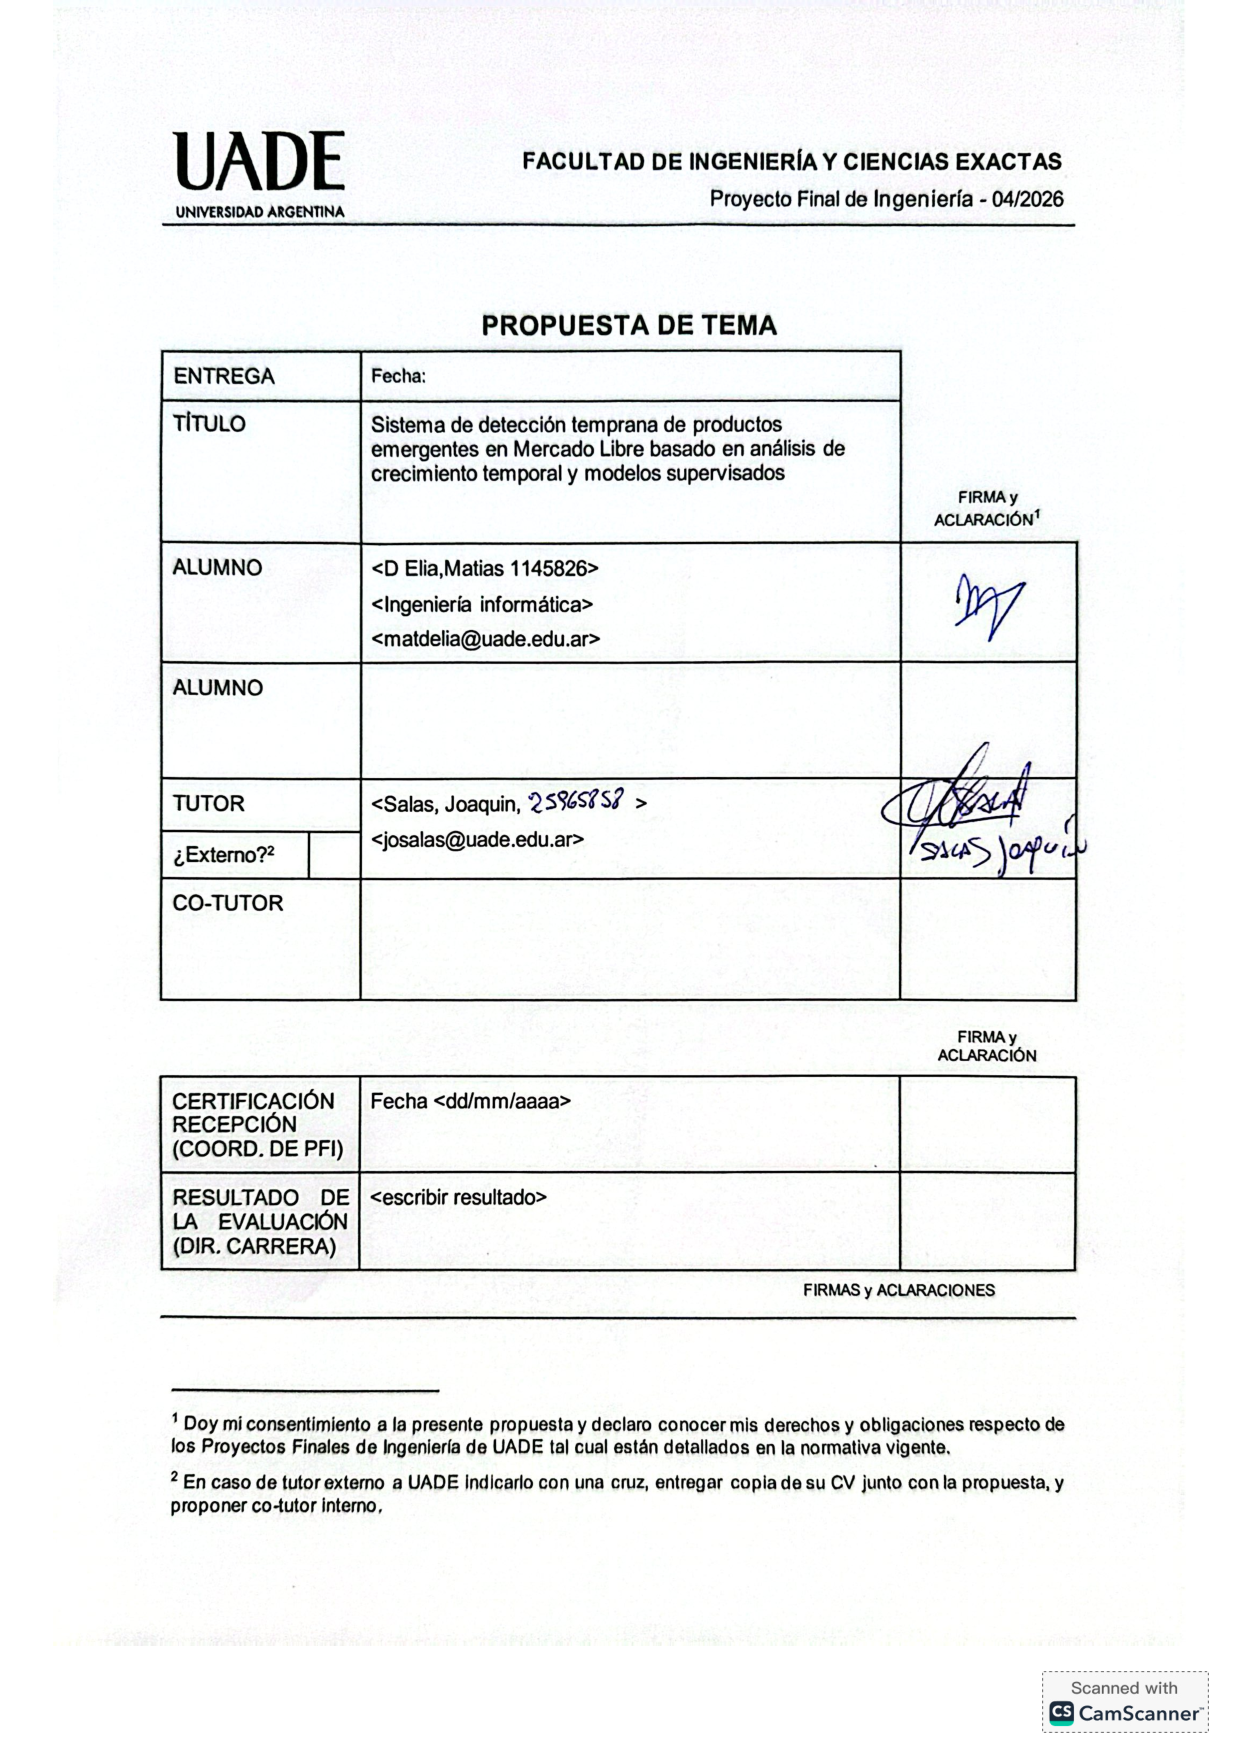
\includepdf[pages=-, pagecommand={\thispagestyle{empty}}]{cover/propuesta_tema.pdf}}
\clearpage

	\chapter{Marco Teórico}\label{chapter01}

El crecimiento del comercio electrónico durante los últimos años produjo una transformación significativa en la manera en que consumidores, vendedores y empresas interactúan dentro de plataformas digitales. Los marketplaces modernos concentran millones de productos, búsquedas y transacciones diarias, generando grandes volúmenes de información capaces de reflejar tendencias de consumo, variaciones de demanda y cambios en el comportamiento del mercado.

En este contexto, la información generada por la actividad de los usuarios dentro de entornos digitales no solo permite describir comportamientos ya ocurridos, sino que también puede funcionar como una señal temprana para anticipar cambios de demanda. En trabajos como el de \textcite{KulkarniKannanMoe2012}, los datos de búsqueda en línea son utilizados para anticipar ventas de productos nuevos, lo que refuerza la utilidad de observar señales digitales antes de que una tendencia se encuentre completamente consolidada.

Dentro de este contexto, Mercado Libre representa uno de los ecosistemas comerciales más importantes de América Latina. Su infraestructura reúne vendedores, compradores y productos pertenecientes a múltiples categorías, convirtiéndose en una fuente extremadamente valiosa de información relacionada con consumo digital y comportamiento comercial.

A pesar del gran volumen de información disponible, uno de los principales problemas detectados es la dificultad para identificar productos emergentes de manera temprana. La mayoría de las herramientas actuales únicamente muestran tendencias instantáneas o rankings superficiales, sin construir datasets históricos persistentes capaces de alimentar modelos predictivos o sistemas avanzados de inteligencia comercial.

Como consecuencia, muchos vendedores y emprendedores ingresan tarde a tendencias ya consolidadas, perdiendo oportunidades comerciales debido al aumento de competencia y reducción de márgenes de rentabilidad.

Frente a esta problemática, el presente proyecto propone el desarrollo de una plataforma inteligente capaz de detectar tempranamente productos emergentes mediante la utilización exclusiva de la API oficial de Mercado Libre, mecanismos automatizados de minería de datos y análisis temporal basado en datos históricos construido internamente.

La solución propuesta busca transformar señales dispersas provenientes del marketplace como tendencias, búsquedas, publicaciones, precios y categorías en información estructurada y utilizable para la toma de decisiones comerciales.

En el proyecto, el término ``tendencia'' no se utiliza como sinónimo de ranking instantáneo, sino como una variación observable y sostenida en el tiempo. Cuando se menciona ``búsquedas'', se hace referencia a resultados públicos obtenidos desde endpoints oficiales de búsqueda y no a datos privados de comportamiento de usuarios. Por lo tanto, la detección se apoyará en variables accesibles y registrables como frecuencia de aparición, variación de cantidad de publicaciones, permanencia en listados, evolución de precios, categoría asociada y cambios relativos frente a períodos anteriores.

El enfoque planteado se sostiene sobre tres ejes principales: la recolección automatizada de información accesible desde fuentes oficiales, la construcción progresiva de un histórico propio y el análisis temporal de variables que puedan funcionar como indicios de crecimiento. Esta decisión permite diferenciar el proyecto de una herramienta meramente descriptiva, ya que el valor principal no se encuentra solo en mostrar datos actuales, sino en observar su evolución y detectar comportamientos emergentes.

\section{Concepto central}

Desarrollar una plataforma inteligente capaz de detectar tempranamente productos emergentes en Mercado Libre mediante la recolección automatizada de datos provenientes de su API oficial, la construcción de un dataset histórico propio y el análisis temporal utilizando métricas descriptivas y modelos supervisados de aprendizaje automático.

A los fines del proyecto, un producto emergente será aquel que, durante una ventana temporal definida, presente crecimiento sostenido en frecuencia de aparición, permanencia y/o publicaciones asociadas, con variaciones de precio o categoría que permitan diferenciarlo de aumentos aislados. Esta definición convierte la idea general de tendencia en un conjunto de indicadores medibles a partir del histórico propio.

\section{Decisiones técnicas}

Las decisiones técnicas adoptadas dentro del proyecto responden principalmente a la necesidad de garantizar escalabilidad, automatización, persistencia histórica y capacidad analítica.

Para eso, se plantea una arquitectura basada en APIs REST oficiales, permitiendo acceder a información estructurada y confiable proveniente del marketplace. Asimismo, la construcción de datasets históricos resulta fundamental para realizar análisis temporales y detectar patrones de crecimiento sostenido.

Por otro lado, la incorporación de técnicas de minería de datos permite extraer información relevante a partir de grandes volúmenes de datos, mientras que el uso de modelos supervisados posibilita analizar comportamientos emergentes y diferenciar tendencias reales de variaciones temporales aisladas.

Finalmente, la implementación de dashboards analíticos y mecanismos de monitoreo contribuye a mejorar la visualización de métricas, el seguimiento de tendencias y la disponibilidad operativa de los servicios utilizados.

\section{Alcance}

El proyecto se enfoca exclusivamente en Mercado Libre Argentina utilizando únicamente información obtenida mediante endpoints oficiales autorizados. La plataforma contempla procesos de captura automatizada, construcción de históricos temporales, monitoreo de endpoints y visualización analítica.

El alcance no incluye scraping, acceso a datos privados de usuarios ni predicción directa de ventas internas de Mercado Libre. La plataforma trabajará únicamente con datos disponibles mediante API oficial y con el histórico construido por el propio sistema.

\section{Tecnologías utilizadas}

\subsection{APIs REST}

Las APIs REST constituyen uno de los mecanismos de comunicación más utilizados dentro de arquitecturas distribuidas modernas. Su utilización permite el intercambio estructurado de información entre sistemas mediante protocolos estándar como HTTP.

En el contexto del comercio electrónico, las APIs facilitan el acceso automatizado a información relacionada con productos, búsquedas, tendencias y categorías, permitiendo construir soluciones analíticas basadas en datos externos confiables y actualizados.

La API oficial de Mercado Libre representa la principal fuente de información utilizada dentro del proyecto, ya que permite acceder de manera estructurada a distintos recursos del marketplace mediante autenticación y solicitudes controladas.

\subsection{Minería de Datos}

La minería de datos comprende el conjunto de técnicas orientadas a descubrir patrones, relaciones y comportamientos relevantes dentro de grandes volúmenes de información.

En plataformas de comercio electrónico, estas técnicas permiten identificar productos con crecimiento sostenido, detectar cambios en tendencias de consumo y analizar comportamientos asociados a la demanda del mercado.

Su aplicación resulta especialmente importante en escenarios donde existe una gran cantidad de datos dispersos y dinámicos, ya que posibilita transformar información no estructurada en conocimiento útil para la toma de decisiones.

Dentro del proyecto, la minería de datos constituye uno de los pilares principales para la construcción de históricos y el análisis de productos emergentes.

\subsection{Series Temporales}

Las series temporales representan secuencias de datos organizadas cronológicamente. Su análisis permite estudiar la evolución de determinadas variables a lo largo del tiempo e identificar patrones de crecimiento, estacionalidad y cambios de comportamiento.

En el ámbito del comercio electrónico, el análisis temporal resulta fundamental para comprender cómo evolucionan las tendencias de consumo y detectar variaciones sostenidas en productos o categorías específicas.

Variables como frecuencia de aparición, crecimiento progresivo, cambios de ranking o variaciones de precio pueden utilizarse como indicadores de comportamiento emergente, permitiendo construir métricas orientadas a la detección temprana de tendencias.

Los trabajos sobre predicción de demanda y series temporales, como el de \textcite{LimArikLoeffPfister2021}, muestran la importancia de considerar la evolución histórica de múltiples variables para analizar escenarios de comportamiento futuro.

\subsection{Machine Learning Supervisado}

El aprendizaje automático supervisado permite desarrollar modelos capaces de identificar patrones y realizar clasificaciones a partir de datos previamente etiquetados.

En proyectos orientados al análisis de tendencias, estos modelos pueden utilizarse para reconocer comportamientos asociados a productos emergentes, diferenciar tendencias reales de fluctuaciones temporales y generar estimaciones probabilísticas basadas en datos históricos.

La utilización de variables temporales y métricas descriptivas permite construir modelos con capacidad de aprendizaje progresivo, aportando mayor precisión en la identificación de oportunidades comerciales.

En una primera etapa, el proyecto prioriza métricas descriptivas y reglas de análisis temporal. Posteriormente, esas variables podrán utilizarse como entrada de modelos supervisados, por ejemplo para clasificar productos según su probabilidad de presentar crecimiento sostenido. Esta decisión es consistente con trabajos como el de \textcite{ElalemMaierSeifert2023}, donde se analiza la predicción de productos nuevos con ciclos de vida cortos y disponibilidad limitada de datos históricos.

\section{Stack tecnológico preliminar}

El stack tecnológico se define de manera preliminar para bajar la arquitectura a decisiones más concretas, sin cerrar completamente futuras modificaciones de implementación.

\begin{table}[ht]
	\centering
	\caption{Stack tecnológico preliminar}
	\label{tab:stack}
	\begin{tabularx}{\textwidth}{@{}>{\raggedright\arraybackslash}p{2.6cm} >{\raggedright\arraybackslash}p{4.2cm} X@{}}
		\toprule
		\textbf{Componente} & \textbf{Tecnología propuesta} & \textbf{Justificación} \\
		\midrule
		Frontend & Next.js (React + TypeScript) & Permite construir dashboards web con componentes reutilizables y tipado estático. \\
		Backend & Next.js (API Routes) + TypeScript & Facilita exponer servicios REST y conectar la lógica de negocio con el análisis de datos. \\
		Captura de datos & Node.js + consultas a API oficial & Permite automatizar solicitudes controladas a Mercado Libre sin depender de scraping externo. \\
		Persistencia & PostgreSQL (Supabase) + Prisma ORM & Permite almacenar información estructurada e históricos temporales con consultas relacionales. \\
		Análisis & Python (Pandas + Scikit-Learn) para la etapa de ML & Herramientas ampliamente utilizadas para procesamiento de datos y modelos supervisados. \\
		Visualización & Dashboard web & Permite presentar tendencias, métricas y alertas en una interfaz comprensible para el usuario. \\
		\bottomrule
	\end{tabularx}
\end{table}

\section{Evolución de las decisiones técnicas}

Durante la implementación del prototipo, el stack preliminar fue ajustado: el backend y la captura de datos se desarrollaron finalmente sobre Next.js (API Routes) y Node.js, unificando frontend y backend en un único lenguaje (TypeScript) y un único despliegue, lo que reduce la complejidad operativa del proyecto. La capa de persistencia (PostgreSQL, gestionada mediante el ORM Prisma) y la arquitectura general de componentes (captura \(\rightarrow\) base histórica \(\rightarrow\) motor analítico \(\rightarrow\) API \(\rightarrow\) dashboard) se mantienen sin cambios: se modificó la herramienta de implementación, no el diseño. Python (Pandas + Scikit-Learn) queda reservado para el motor analítico y de Machine Learning de la etapa siguiente, que se integrará leyendo directamente la base histórica PostgreSQL.

\section{Arquitectura General}

La arquitectura del sistema se encuentra organizada en distintos componentes que trabajan de manera integrada para permitir la captura, procesamiento, almacenamiento y visualización de información relacionada con tendencias comerciales.

El frontend cumple la función de representar la información de manera visual e intuitiva, permitiendo interpretar tendencias, métricas temporales y variaciones de comportamiento de los productos. La visualización de datos resulta fundamental para facilitar la toma de decisiones y transformar grandes volúmenes de información en indicadores comprensibles para el usuario (ver Figura~\ref{fig:diagrama-componentes}, \emph{Dashboard (React)} dentro del Carril 2).

Por otro lado, el backend actúa como el componente encargado de administrar el procesamiento general de la plataforma. Su función principal consiste en organizar la información obtenida, coordinar los distintos procesos internos y garantizar el correcto funcionamiento de la lógica del sistema (ver Figura~\ref{fig:diagrama-componentes}, \emph{API REST (API Routes)} dentro del Carril 2).

El motor de minería de datos representa uno de los elementos centrales del proyecto, ya que permite automatizar la obtención y análisis de información proveniente del marketplace. Su importancia radica en la capacidad de detectar patrones, registrar cambios temporales y construir históricos que luego pueden utilizarse para identificar comportamientos emergentes (ver Figura~\ref{fig:diagrama-componentes}, subsistema \emph{Captura automatizada -- Carril 1}).

La persistencia de datos cumple un rol clave dentro de la plataforma debido a que posibilita almacenar información histórica de manera organizada y continua. Mantener registros temporales permite realizar comparaciones, analizar evolución de tendencias y generar bases de información útiles para futuros modelos analíticos (ver Figura~\ref{fig:diagrama-componentes}, componente \emph{Base Histórica}; el detalle de las tablas se muestra en la Figura~\ref{fig:diagrama-er}).

Finalmente, el monitoreo contribuye a garantizar estabilidad y disponibilidad dentro del sistema, permitiendo controlar el comportamiento de los servicios utilizados y detectar posibles interrupciones o variaciones que puedan afectar la recolección de información (ver Figura~\ref{fig:diagrama-componentes}, \emph{probe\_endpoints.js} dentro del Carril 1).

La arquitectura opera además en dos carriles complementarios. El primero es el carril de captura en segundo plano: los procesos programados que construyen el histórico de manera sistemática y controlada, tres veces por día. El segundo es un carril de consulta en tiempo real: desde el dashboard, el usuario puede buscar productos puntuales consultando la API oficial en vivo, sin esperar a la próxima corrida de captura. Esta separación protege la recolección sistemática (cuyo ritmo está calibrado para respetar los límites de la API) de la carga variable de las consultas interactivas, y permite contrastar el histórico propio con el estado instantáneo del marketplace (ambos carriles se distinguen en la Figura~\ref{fig:diagrama-componentes}).

\subsection{Diagrama de componentes propuesto}

\begin{figure}[ht]
	\centering
	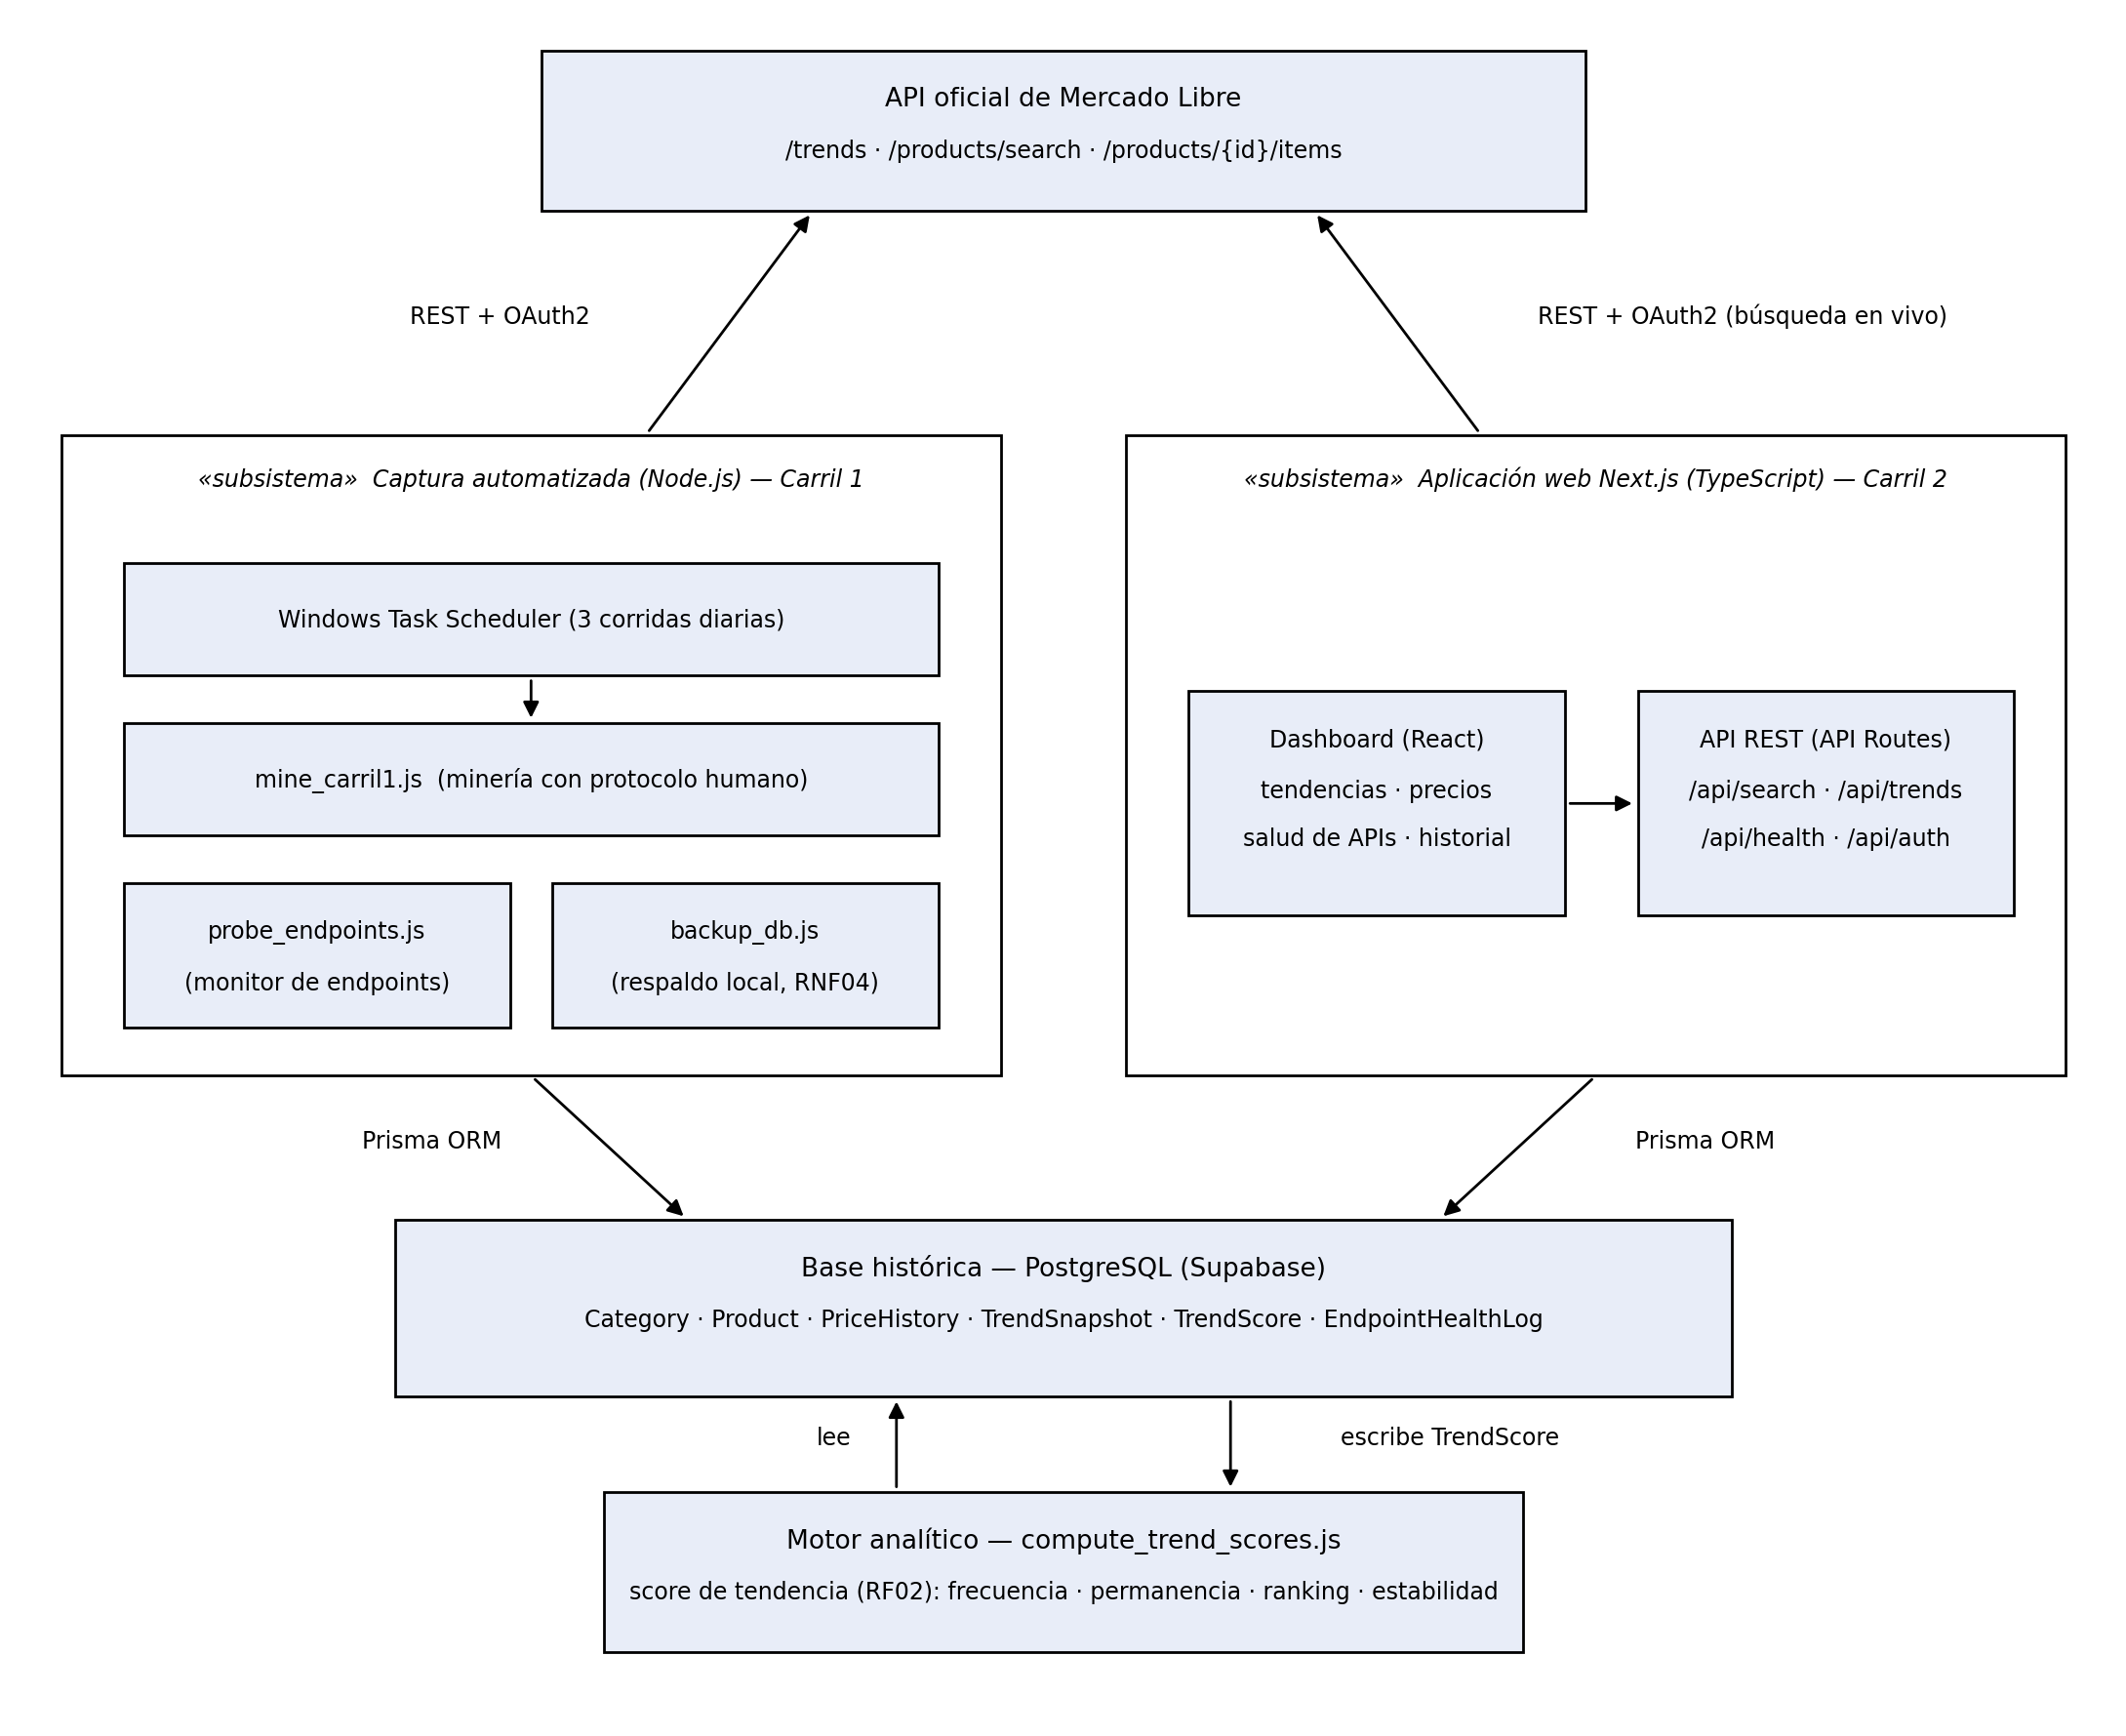
\includegraphics[width=0.95\textwidth]{./images/diagramas/diagrama_componentes.png}
	\caption{Diagrama de componentes del sistema.}
	\label{fig:diagrama-componentes}
\end{figure}

El flujo de datos comienza con consultas periódicas a la API oficial de Mercado Libre. Luego, la información recolectada se almacena en una base histórica. A partir de ese histórico, el motor analítico calcula métricas temporales que permiten identificar productos con crecimiento sostenido o cambios relevantes. Finalmente, el backend expone esos resultados para que el dashboard los presente de manera visual (flujo completo en la Figura~\ref{fig:diagrama-componentes}).

\subsection{Diagrama de Clases (UML)}

El diagrama de clases representa las principales entidades del sistema y sus relaciones (ver Figura~\ref{fig:diagrama-uml}).

\begin{figure}[ht]
	\centering
	
\includegraphics[width=0.85\textwidth]{./images/diagramas/diagrama_clases_uml.png}
	\caption{Diagrama de clases UML del sistema.}
	\label{fig:diagrama-uml}
\end{figure}

\subsection{Modelo de Datos -- Diagrama Entidad-Relación}

El modelo de datos se implementa sobre PostgreSQL. El diagrama Entidad-Relación muestra las tablas principales y sus relaciones (1:N) (ver Figura~\ref{fig:diagrama-er}).

\begin{figure}[ht]
	\centering
	
\includegraphics[width=0.9\textwidth]{./images/diagramas/diagrama_er.png}
	\caption{Diagrama Entidad-Relación del modelo de datos.}
	\label{fig:diagrama-er}
\end{figure}

\section{Modelos y Arquitecturas Aplicables}

El desarrollo de plataformas inteligentes orientadas al análisis de tendencias requiere la utilización de arquitecturas capaces de procesar información de manera distribuida, escalable y organizada. En este contexto, los modelos basados en arquitecturas cliente-servidor y servicios desacoplados permiten separar responsabilidades entre captura de datos, procesamiento, persistencia y visualización de información.

La arquitectura cliente-servidor constituye uno de los modelos más utilizados dentro de aplicaciones modernas debido a su capacidad para dividir el sistema en componentes especializados. El frontend se encarga de la interacción con el usuario y visualización de resultados, mientras que el backend administra la lógica de negocio, procesamiento de información y comunicación con servicios externos.

Dentro del proyecto, este enfoque permite organizar la plataforma en módulos independientes capaces de trabajar de manera coordinada. La captura automatizada de información proveniente de Mercado Libre se realiza mediante procesos específicos de minería de datos, mientras que el backend administra el almacenamiento histórico, la generación de métricas y el monitoreo de disponibilidad de endpoints.

Además, el uso de APIs REST como mecanismo de integración favorece la interoperabilidad entre sistemas y simplifica el intercambio de información estructurada mediante solicitudes HTTP y respuestas en formato JSON. Este modelo de comunicación se consolidó como estándar en aplicaciones distribuidas debido a su flexibilidad, escalabilidad y facilidad de integración con múltiples tecnologías.

Por otra parte, la utilización de arquitecturas basadas en procesamiento de datos temporales resulta especialmente relevante en sistemas de análisis predictivo. La construcción progresiva de datasets históricos permite transformar eventos aislados en información acumulativa capaz de reflejar patrones de crecimiento, cambios de comportamiento y tendencias emergentes.

En proyectos orientados a inteligencia comercial, estas arquitecturas permiten incorporar posteriormente modelos de aprendizaje automático, motores analíticos y dashboards interactivos sin necesidad de rediseñar completamente la estructura principal del sistema. De esta manera, la arquitectura no solo cumple una función técnica, sino que también condiciona la capacidad futura de expansión y evolución de la plataforma.

\section{Métricas y Análisis Temporal}

El análisis temporal constituye uno de los componentes centrales en sistemas orientados a la detección de tendencias y comportamiento emergente. A diferencia de los análisis estáticos, las métricas temporales permiten observar cómo evolucionan determinados fenómenos a lo largo del tiempo, facilitando la identificación de patrones de crecimiento, estacionalidad y cambios abruptos en la demanda.

Dentro del comercio electrónico, las variaciones temporales representan señales fundamentales para comprender el comportamiento del mercado. Factores como el aumento sostenido de publicaciones, la frecuencia de aparición de determinados productos, las variaciones de precio y los cambios de ranking pueden reflejar el inicio de nuevas tendencias comerciales antes de que se consoliden masivamente.

En este proyecto, el análisis temporal se basa principalmente en la construcción de datos históricos propios obtenidos mediante la API oficial de Mercado Libre. La persistencia de información cronológica permite comparar comportamientos entre distintos períodos y detectar productos con crecimiento sostenido respecto de su categoría.

Las métricas descriptivas constituyen la primera aproximación para interpretar estos datos. Indicadores como frecuencia de aparición, crecimiento porcentual, permanencia dentro de tendencias y evolución de precios permiten generar una representación cuantitativa del comportamiento de cada producto dentro del marketplace.

A su vez, estas métricas funcionan como base para futuros modelos supervisados de Machine Learning, ya que las variables históricas permiten entrenar algoritmos capaces de diferenciar tendencias reales de aumentos temporales de popularidad. De esta manera, el análisis temporal no solo aporta información descriptiva, sino también capacidades predictivas orientadas a mejorar la toma de decisiones comerciales.

Finalmente, el uso de métricas históricas contribuye a reducir la dependencia de rankings instantáneos o tendencias superficiales, permitiendo construir una visión más consistente y contextualizada del comportamiento del mercado digital.

La detección temprana no se define por la aparición aislada de un producto en un ranking, sino por la repetición de señales durante un período determinado. Por ese motivo, el proyecto prioriza métricas que permitan observar continuidad, intensidad y variación temporal.

\subsection{Métricas preliminares}

\begin{table}[ht]
	\centering
	\caption{Métricas preliminares}
	\label{tab:metricas}
	\begin{tabularx}{\textwidth}{@{}>{\raggedright\arraybackslash}p{3cm} >{\raggedright\arraybackslash}p{4cm} p{1.8cm} X@{}}
		\toprule
		\textbf{Métrica} & \textbf{Descripción} & \textbf{Tipo} & \textbf{Utilidad para el proyecto} \\
		\midrule
		Frecuencia de aparición & Cantidad de veces que un producto aparece en consultas o registros temporales. & Descriptiva & Permite observar presencia sostenida. \\
		Crecimiento porcentual & Variación entre períodos consecutivos. & Descriptiva & Permite identificar aumentos relevantes. \\
		Permanencia en tendencias & Cantidad de períodos en los que el producto mantiene visibilidad. & Descriptiva & Ayuda a diferenciar señales aisladas de tendencias sostenidas. \\
		Evolución de precios & Cambios de precio registrados a lo largo del tiempo. & Descriptiva & Permite analizar comportamiento comercial y competencia. \\
		Variación de publicaciones & Cambios en la cantidad de publicaciones asociadas a un producto o categoría. & Predictiva & Puede indicar aumento de oferta o interés comercial. \\
		Indicador compuesto & Combinación ponderada de métricas anteriores. & Propuesta & Podría utilizarse como base para clasificar productos emergentes. \\
		\bottomrule
	\end{tabularx}
\end{table}
 % Marco Teórico
	\chapter{Estado del Arte}\label{chapter02}

\section{Relevamiento de principales aplicaciones en Argentina}

A continuación se presenta un relevamiento de las principales aplicaciones y sitios web orientados a vendedores de Mercado Libre en Argentina, clasificados según su tipo y funcionalidad.

\begin{table}[ht]
	\centering
	\caption{Relevamiento de principales aplicaciones en Argentina}
	\label{tab:relevamiento}
	\small
	\begin{tabularx}{\textwidth}{@{}>{\raggedright\arraybackslash}p{1.8cm} >{\raggedright\arraybackslash}p{1.9cm} >{\raggedright\arraybackslash}p{2.3cm} >{\raggedright\arraybackslash}p{1.7cm} >{\raggedright\arraybackslash}p{2.1cm} X@{}}
		\toprule
		\textbf{Herramienta} & \textbf{Tipo} & \textbf{Funcionalidades principales} & \textbf{Público objetivo} & \textbf{Limitaciones} & \textbf{Diferencia con el proyecto} \\
		\midrule
		Real Trends & Todo en uno & Gestión de publicaciones, competencia, precios y respuestas automáticas. & Vendedores medianos y grandes. & Se orienta a operación y optimización de ventas existentes. & El proyecto se enfoca en detección temprana mediante históricos propios. \\
		UpSeller ERP & ERP / multicanal & Inventario, publicaciones, pedidos, análisis competitivo y sincronización. & Empresas con operación multicanal. & Predomina la gestión operativa e inventario. & El proyecto prioriza análisis temporal de productos emergentes. \\
		Administrado & Gestión integral & Ventas, stock, atención al cliente, facturación y métricas. & Vendedores que buscan centralizar cuentas. & No está centrado en forecasting ni señales tempranas. & La propuesta busca identificar oportunidades antes de su consolidación. \\
		Ecomm-App & Analítica y gestión & Inventario, métricas de venta y mapas de actividad. & Vendedores en crecimiento. & Trabaja con métricas más retrospectivas. & El proyecto construye históricos para análisis evolutivo. \\
		MercadoBot & Automatización & Respuestas automáticas, mensajería y alertas de stock. & Vendedores que priorizan atención al cliente. & No analiza tendencias de mercado. & La propuesta se orienta a inteligencia comercial predictiva. \\
		Herramientas nativas de Mercado Libre & Panel interno & Métricas básicas, publicaciones y desempeño del vendedor. & Todos los vendedores. & Información limitada y principalmente descriptiva. & El proyecto agrega almacenamiento histórico y análisis temporal propio. \\
		\bottomrule
	\end{tabularx}
\end{table}

La brecha identificada se encuentra en que las soluciones relevadas se orientan principalmente a gestión, automatización, stock, atención al cliente o análisis de resultados ya ocurridos. En cambio, el presente proyecto busca cubrir un espacio más específico: la detección temprana de productos emergentes mediante histórico propio, análisis temporal y modelos supervisados.

Esta brecha justifica el desarrollo de una plataforma propia capaz de detectar tempranamente productos emergentes mediante la recolección automatizada de datos vía API oficial de Mercado Libre, la construcción de un dataset histórico estructurado y el análisis temporal con modelos supervisados de aprendizaje automático.

\subsection{Tabla comparativa de alternativas}

Se compara la propuesta con herramientas y plataformas existentes que abordan problemas similares de detección de tendencias o seguimiento de precios.

\begin{table}[ht]
	\centering
	\caption{Tabla comparativa de alternativas}
	\label{tab:comparativa}
	\small
	\begin{tabularx}{\textwidth}{@{}>{\raggedright\arraybackslash}p{2.2cm} >{\raggedright\arraybackslash}p{2.6cm} >{\raggedright\arraybackslash}p{2.7cm} >{\raggedright\arraybackslash}p{2.7cm} X@{}}
		\toprule
		\textbf{Herramienta} & \textbf{Enfoque} & \textbf{Tecnología/ Fuente} & \textbf{Limitación} & \textbf{Diferencial del proyecto} \\
		\midrule
		Google Trends & Tendencias de búsqueda general & Datos de búsqueda de Google & No vincula con precio ni disponibilidad real de productos & Usa señales directas del marketplace (precio, publicaciones, categoría) \\
		Keepa / CamelCamelCamel & Histórico de precios (Amazon) & Scraping de Amazon & Sólo Amazon, no aplica a Mercado Libre ni analiza tendencia emergente & Enfocado en Mercado Libre Argentina con score de tendencia propio \\
		Trendyol/ML Insights internos & Analítica interna de marketplace & Datos propios de la plataforma & No accesible para vendedores externos & Accesible a cualquier vendedor mediante API oficial pública \\
		Sistema propuesto & Detección temprana de productos en tendencia & API oficial ML + PostgreSQL + modelos analíticos & Depende de límites de la API oficial & Combina histórico propio, score de tendencia y alertas tempranas \\
		\bottomrule
	\end{tabularx}
\end{table}

\section{Antecedentes académicos y trabajos relacionados}

Como parte del relevamiento bibliográfico, se analizaron distintos trabajos académicos relacionados con análisis predictivo, tendencias digitales y detección temprana de comportamiento de consumo en entornos de comercio electrónico. La incorporación de estos antecedentes resulta importante porque permiten fundamentar teóricamente la lógica utilizada dentro del proyecto y validar que el uso de señales tempranas, históricos temporales y modelos analíticos representa una línea de investigación actualmente utilizada dentro del área de inteligencia comercial y análisis de datos.

Uno de los trabajos más relevantes analizados fue \emph{``Using Online Search Data to Forecast New Product Sales''} de \textcite{KulkarniKannanMoe2012}. Este paper plantea que los patrones de búsqueda online pueden utilizarse como indicadores tempranos capaces de anticipar el comportamiento futuro de determinados productos antes de que la tendencia se encuentre completamente consolidada. Lo más destacable del trabajo es que demuestra cómo ciertas señales digitales generadas por los usuarios pueden transformarse en variables predictivas útiles para detectar interés creciente dentro del mercado.

Este enfoque guarda una relación directa con el objetivo principal del presente proyecto, ya que la plataforma propuesta busca precisamente identificar comportamientos emergentes mediante señales obtenidas desde Mercado Libre, como tendencias, frecuencia de aparición, evolución temporal y variaciones dentro del marketplace. Aunque el estudio se desarrolla sobre otro tipo de entorno digital, la lógica metodológica resulta totalmente aplicable al problema planteado, especialmente en lo relacionado con la utilización de datos tempranos como indicadores de posibles oportunidades comerciales futuras.

Por otro lado, también se analizó el paper \emph{``A Machine Learning-Based Framework for Forecasting Sales of New Products with Short Life Cycles Using Deep Neural Networks''} de \textcite{ElalemMaierSeifert2023}. Este trabajo resultó relevante debido a que aborda un problema muy similar al del proyecto, cómo analizar y predecir el comportamiento de productos nuevos cuando todavía existe poca información histórica disponible.

Uno de los aspectos más interesantes del paper es que no se limita únicamente al uso de redes neuronales profundas, sino que además compara distintos enfoques estadísticos y modelos de aprendizaje automático para evaluar cuál se adapta mejor a escenarios con históricos limitados. Los autores demuestran que, en determinados contextos, modelos tradicionales pueden incluso obtener mejores resultados que arquitecturas más complejas, lo cual aporta una visión metodológica más realista y sólida desde el punto de vista académico.

Este trabajo resulta especialmente útil para el proyecto porque respalda la idea de comenzar inicialmente con métricas descriptivas y análisis temporal antes de avanzar hacia modelos supervisados más complejos. Además, aporta fundamentos concretos sobre cómo trabajar con productos emergentes o tendencias nuevas que todavía no poseen grandes volúmenes de información histórica acumulada, situación que representa uno de los principales desafíos dentro de plataformas de detección temprana de tendencias.

\subsection*{Schaer, Kourentzes y Fildes (2019)}

El trabajo de \textcite{SchaerKourentzesFildes2019}, vinculado con demand forecasting e información generada por usuarios en línea, resulta relevante porque analiza cómo incorporar señales digitales externas dentro de modelos de predicción de demanda. Este antecedente permite reforzar la idea de que los datos generados en entornos digitales pueden aportar valor predictivo cuando se los organiza y analiza temporalmente.

La relación con el proyecto se encuentra en qué Mercado Libre funciona como una fuente de señales comerciales dinámicas. A través de variables como publicaciones, precios, categorías y frecuencia de aparición, es posible construir una base de información que no dependa únicamente de rankings instantáneos, sino de la evolución del comportamiento de mercado.

El aporte metodológico de este antecedente es que permite trasladar el foco desde la venta ya ocurrida hacia señales previas de interés comercial. Para este proyecto, esa lógica se adapta al uso de variables observables en Mercado Libre, reemplazando el análisis de datos generales de búsqueda por registros temporales derivados de consultas oficiales, publicaciones, precios y categorías del marketplace.

\subsection*{Lim, Arık, Loeff y Pfister (2021)}

\textcite{LimArikLoeffPfister2021} presentan los Temporal Fusion Transformers como una arquitectura orientada a predicción de series temporales multi-horizonte e interpretable. Aunque el proyecto no contempla implementar esta arquitectura en su primera versión, el antecedente resulta útil porque muestra la importancia de combinar múltiples variables temporales para mejorar el análisis predictivo.

Este trabajo se toma como respaldo para futuras extensiones del sistema, especialmente si el prototipo evoluciona hacia modelos de forecasting más complejos. En la etapa actual, su aporte principal es conceptual: confirma que la predicción temporal requiere históricos consistentes y variables bien definidas.

Este antecedente no implica que el proyecto deba implementar Temporal Fusion Transformers en su primera versión, ya que requiere mayor volumen histórico y mayor complejidad técnica. Sin embargo, sí refuerza la decisión de diseñar desde el inicio una base temporal ordenada, con variables consistentes y preparadas para futuras extensiones predictivas.

\subsection*{Salamai, Ageeli y El-kenawy (2022)}

El trabajo de \textcite{SalamaiAgeeliElkenawy2022} aborda el uso de modelos basados en LSTM para analizar comportamientos temporales en comercio electrónico. Este tipo de arquitectura permite capturar dependencias de largo plazo y resulta relevante para comprender cómo pueden modelarse patrones de comportamiento cuando existe suficiente información histórica.

En relación con el presente proyecto, este antecedente permite justificar la construcción de un dataset histórico propio como condición previa para cualquier modelo predictivo más avanzado. Sin una base temporal consistente, la aplicación de modelos supervisados o de aprendizaje profundo tendría un valor limitado.

El vínculo con la propuesta se encuentra en que los modelos de aprendizaje profundo solo son aplicables cuando existe una secuencia histórica suficiente. Por eso, este antecedente no se utiliza como solución inmediata, sino como justificación académica de la necesidad de capturar datos de forma periódica y persistente antes de avanzar hacia modelos más complejos.

En conjunto, estos trabajos académicos permiten reforzar conceptualmente el proyecto, ya que validan la importancia de utilizar señales digitales tempranas, históricos temporales y modelos analíticos como herramientas para anticipar comportamientos futuros dentro de ecosistemas de comercio electrónico. Asimismo, sirven como respaldo metodológico para la construcción de una plataforma orientada al análisis inteligente de productos emergentes utilizando información proveniente exclusivamente de la API oficial de Mercado Libre.
 % Estado del Arte
	\chapter{Requerimientos}\label{chapter03}

A continuación se detallan los requerimientos funcionales y no funcionales del sistema, junto con las historias de usuario que guían el desarrollo del producto.

\section{Historias de Usuario}

\begin{itemize}
	\item HU01 -- Como vendedor, quiero visualizar un ranking de productos en tendencia por categoría para decidir qué publicar.
	\item HU02 -- Como vendedor, quiero recibir una alerta cuando un producto que sigo empiece a crecer en tendencia, sin tener que entrar a revisar el dashboard.
	\item HU03 -- Como comprador, quiero ver el histórico de precio de un producto antes de comprarlo.
	\item HU04 -- Como usuario, quiero filtrar productos por categoría, rango de fecha y precio.
	\item HU05 -- Como administrador, quiero configurar la frecuencia de captura de datos desde la API de Mercado Libre (implementada mediante tareas programadas del sistema operativo: tres corridas diarias parametrizables).
	\item HU06 -- Como cliente, quiero crear una cuenta para acceder a las funciones del nivel pago del modelo freemium (historial completo, exportación y alertas).
	\item HU07 -- Como cliente, quiero seguir un producto puntual desde el ranking, para que el sistema me avise si empieza a crecer en vez de tener que revisarlo yo.
\end{itemize}

\section{Requerimientos Funcionales}

\begin{enumerate}
	\item RF01 -- El sistema debe capturar periódicamente datos de productos desde la API oficial de Mercado Libre.
	\item RF02 -- El sistema debe calcular un score de tendencia por producto en base a variables temporales.
	\item RF03 -- El sistema debe permitir filtrar y ordenar productos por categoría, score, variación de precio, rango de precio y rango de fecha.
	\item RF04 -- El sistema debe exponer los resultados mediante una API REST (Next.js API Routes).
	\item RF05 -- El dashboard debe mostrar gráficos de evolución temporal por producto y categoría.
	\item RF06 -- El sistema debe permitir exportar el listado de productos en tendencia (CSV).
	\item RF07 -- El sistema debe exponer, para cada producto, la probabilidad estimada por el modelo de Machine Learning supervisado (Sección~\ref{sec:ml-resultados}) de que su score siga creciendo.
	\item RF08 -- El sistema debe permitir a un usuario crear una cuenta y autenticarse, para diferenciar el nivel gratuito del nivel pago del modelo freemium (Sección~\ref{sec:modelo-negocio}).
	\item RF09 -- El sistema debe permitir a un cliente autenticado seguir un producto puntual y generar una alerta cuando su score cruce el umbral de crecimiento (HU07).
\end{enumerate}

\section{Requerimientos No Funcionales}

\begin{enumerate}
	\item RNF01 -- La captura de datos no debe exceder los límites de rate-limit de la API oficial de Mercado Libre.
	\item RNF02 -- El dashboard debe responder consultas en menos de 3 segundos sobre el dataset histórico. El modelo de datos incluye índices en PostgreSQL (productId, timestamp, categoryId) diseñados para sostener ese tiempo de respuesta a medida que el histórico escala.
	\item RNF03 -- El backend debe poder desplegarse en plataformas cloud con escalado gestionado. Actualmente se despliega en Render con build reproducible (generación de Prisma Client en postinstall).
	\item RNF04 -- Los datos históricos deben persistirse con respaldo (backup) periódico.
	\item RNF05 -- Las credenciales y tokens de acceso (OAuth2 de Mercado Libre) deben gestionarse exclusivamente del lado servidor, sin exponerse nunca al cliente, con renovación automática de tokens.
	\item RNF06 -- El panel administrativo (\texttt{/admin}) no debe ser accesible sin autenticación, dado que expone información operativa interna (logs de minería, estado de endpoints).
	\item RNF07 -- Las contraseñas de los usuarios deben almacenarse con hash seguro (nunca en texto plano ni reversible).
\end{enumerate}

\section{Matriz de trazabilidad}\label{sec:trazabilidad}

La siguiente matriz vincula cada requerimiento con su estado real de implementación al cierre de este hito y con la evidencia concreta que lo respalda, medida sobre el sistema en producción (ver evidencia cuantitativa detallada en la Sección~\ref{sec:evidencia-cuantitativa}).

\begin{longtable}{@{}>{\raggedright\arraybackslash}p{1.6cm} >{\raggedright\arraybackslash}p{2.6cm} >{\raggedright\arraybackslash}p{7.8cm} >{\raggedright\arraybackslash}p{2.1cm}@{}}
	\caption{Matriz de trazabilidad de requerimientos} \label{tab:trazabilidad} \\
	\toprule
	\textbf{Req.} & \textbf{Estado} & \textbf{Evidencia} & \textbf{Sección} \\
	\midrule
	\endfirsthead
	\toprule
	\textbf{Req.} & \textbf{Estado} & \textbf{Evidencia} & \textbf{Sección} \\
	\midrule
	\endhead
	RF01 & Implementado & 274 productos y 5717 apariciones capturados en 71 días de operación continua (14/7 al 23/9/2026), en $\sim$203 sesiones de minería estimadas. & Sec.~\ref{sec:evidencia-cuantitativa}, Fig.~\ref{fig:diagrama-componentes} \\
	RF02 & Implementado & 11573+ scores calculados y persistidos con desglose completo. Fórmula, pesos y ejemplo real documentados. Desde el 23/09/2026 el componente de estabilidad se calcula sobre el precio promedio entre vendedores activos (no el más barato); verificado con una corrida real de minería, 12 productos con datos de múltiples vendedores cargados. & Sec.~\ref{sec:score-formal} \\
	RF03 & Implementado & Filtro por categoría, precio (mín./máx.) y orden por score/variación en el ranking; filtro por rango de fecha (7/30 días/todo) en el gráfico de evolución. & Fig.~\ref{fig:demo-score} \\
	RF04 & Implementado & 5 endpoints REST en producción (\texttt{/api/trend-scores}, \texttt{/api/health}, \texttt{/api/status}, \texttt{/api/search}, \texttt{/api/trends}), más los de cuentas y alertas (\texttt{/api/account/*}, \texttt{/api/watchlist}, \texttt{/api/alerts}). & Sec.~\ref{sec:evidencia-cuantitativa} \\
	RF05 & Implementado & Gráfico de evolución del score de tendencia por producto y panel de tendencias desglosado por categoría, ambos en el dashboard. & Fig.~\ref{fig:demo-evolucion} \\
	RF06 & Implementado & Exportación a CSV del ranking filtrado, disponible en el dashboard (nivel pago, Sección~\ref{sec:modelo-negocio}). & Fig.~\ref{fig:demo-score} \\
	RF07 & Implementado & Columna ``Prob. ML'' en el ranking con la probabilidad calculada por el checkpoint del modelo supervisado, cargada para los 227 productos con score. & Sec.~\ref{sec:ml-resultados} \\
	RF08 & Implementado & Registro y login con contraseña hasheada (bcrypt) y sesión firmada (JWT); nivel gratuito vs. pago diferenciado en el dashboard. & Sec.~\ref{sec:modelo-negocio} \\
	RF09 & Implementado & Botón de seguir por producto (requiere cuenta) y bandeja de alertas en \texttt{/alerts}, generadas al cruzar el umbral de crecimiento. & -- \\
	RNF01 & Implementado & Sin bloqueos por rate-limit en 71 días de operación; los únicos 2 endpoints bloqueados lo están por política de Mercado Libre, no por exceso de solicitudes. & Sec.~\ref{sec:evidencia-cuantitativa} \\
	RNF02 & Implementado & Medido en producción el 21/09/2026, tras acotar la consulta a las últimas 2 mediciones por producto: \texttt{/api/trend-scores} responde en 1,7--2,9\,s en caliente, dentro del objetivo de 3\,s (antes: 6,3--7,6\,s). Detalle de la corrección y su verificación en la Sección~\ref{sec:pruebas}. & Sec.~\ref{sec:evidencia-cuantitativa}, \ref{sec:pruebas} \\
	RNF03 & Implementado & Desplegado en Render, con build reproducible (generación de Prisma Client en \texttt{postinstall}). & -- \\
	RNF04 & Implementado & Respaldo automático (\texttt{backup\_db.js}) ejecutado al final de cada corrida de minería. & -- \\
	RNF05 & Implementado & Tokens OAuth2 persistidos server-side (tabla \texttt{OAuthToken}), con renovación automática cuando faltan menos de 5 minutos para expirar. & -- \\
	RNF06 & Implementado & \texttt{/admin} protegido por un \emph{proxy} (\texttt{src/proxy.ts}) que exige sesión con rol administrador; antes de esta corrección era accesible sin ninguna autenticación. & -- \\
	RNF07 & Implementado & Contraseñas hasheadas con bcrypt (factor de costo 10) antes de persistirse; nunca se guarda ni se loguea la contraseña en texto plano. & -- \\
	\bottomrule
\end{longtable}

Las historias de usuario se consideran implementadas de forma directa cuando su(s) RF asociado(s) están implementados: HU01 (RF01--RF03), HU03 (RF05), HU04 (RF03) y HU05 (RF01). HU02 y HU07 quedan cubiertas por RF09 (seguir un producto y recibir una alerta in-app cuando cruza el umbral de crecimiento) -- con una limitación reconocida: la alerta hoy se ve en \texttt{/alerts} dentro de la aplicación, pero todavía no se envía por email o push, porque eso requiere dar de alta una cuenta en un proveedor externo de correo (Sección~\ref{sec:alcance}). HU06 queda cubierta por RF08.

\section{Metodología de desarrollo}\label{sec:metodologia}

El desarrollo del proyecto se llevó adelante bajo un enfoque ágil de tipo Kanban: ciclos cortos e incrementales de trabajo, integración continua hacia el entorno de producción y ciclos de feedback frecuentes con el tutor, en lugar de iteraciones de duración fija (\emph{sprints}) cerradas de antemano y definidas por adelantado. \textcite{BeckEtAl2001} definen los principios centrales de este tipo de metodologías -- entrega temprana y continua de software funcionando, e incorporación del cambio incluso en etapas avanzadas del desarrollo -- que se reflejan directamente en la forma de trabajo adoptada en este proyecto.

Esta elección se justifica por tres motivos concretos, verificables en el historial de control de versiones del proyecto:

\begin{itemize}
	\item \textbf{Incrementos pequeños y frecuentes}: 63 \emph{commits} entre el 21 de abril y el 31 de agosto de 2026 (aproximadamente cuatro meses y medio), cada uno acotado a un cambio puntual -- una corrección, una funcionalidad o un ajuste de documentación -- en lugar de entregas grandes y espaciadas.
	\item \textbf{Integración continua}: cada incremento se despliega automáticamente al entorno de producción en Render ante cada cambio en la rama principal (RNF03, Sección~\ref{sec:trazabilidad}), permitiendo validar el sistema en condiciones reales en vez de acumular trabajo sin probar.
	\item \textbf{Reorganización del trabajo en respuesta a feedback}: el plan de tareas se ajustó explícitamente en más de una ocasión a partir de devoluciones del tutor -- documentadas tras la entrega del 25\,\% y nuevamente tras la del 50\,\% --, incorporando esos cambios como parte del flujo normal de trabajo en lugar de tratarlos como una fase separada de corrección final.
\end{itemize}

Se descartó una metodología estructurada de tipo cascada porque el proyecto combina componentes con distinto grado de incertidumbre: el pipeline de captura y el dashboard tenían requerimientos claros desde el inicio, mientras que el diseño del score de tendencia y, más adelante, el del modelo de Machine Learning supervisado (Sección~\ref{sec:evolucion-tecnica}) se fueron ajustando a medida que se disponía de más datos reales -- algo que un enfoque secuencial con etapas cerradas de antemano no habría permitido sin retrabajo significativo.

\section{Viabilidad legal y técnica}

El proyecto no aborda una temática sensible en términos legales -- no procesa datos de salud, alimentación ni pone en riesgo la vida de los usuarios --: los datos de producto (precios, categorías, publicaciones) provienen exclusivamente de la API oficial de Mercado Libre (Sección~\ref{sec:tecnologias-utilizadas}) y son públicos, sin acceder a información privada de compradores o vendedores de Mercado Libre (Sección~\ref{sec:alcance}). Por ese motivo, no corresponde incluir un descargo de responsabilidad legal específico más allá del cumplimiento de los términos de uso de la API oficial, ya documentado como RNF05 (gestión segura de credenciales OAuth2 exclusivamente del lado servidor, Sección~\ref{sec:trazabilidad}).

Con la incorporación de cuentas de usuario (RF08, Sección~\ref{sec:modelo-negocio}) el sistema sí pasó a recolectar un dato personal propio, no de Mercado Libre: el email de quien se registra. El tratamiento se mantiene acotado a lo estrictamente necesario para el modelo freemium -- solo email y contraseña hasheada (RNF07), sin datos de pago, dirección ni información adicional -- en línea con los principios de minimización de datos de la Ley 25.326 de Protección de Datos Personales. Queda como trabajo pendiente para una eventual operación comercial real redactar una política de privacidad formal.

En cuanto a viabilidad técnica, el proyecto es enteramente de software: no requiere fabricación ni adquisición de hardware específico, dado que se ejecuta sobre infraestructura \emph{cloud} gestionada -- Render para el backend y Supabase para la base de datos PostgreSQL --, ambas con planes ya operativos y verificados en producción (Sección~\ref{sec:evidencia-cuantitativa}). Por lo tanto, este criterio también se da por cumplido sin requerir un análisis adicional de producción o compra de equipamiento.
 % Requerimientos
	\chapter{Mockups}\label{chapter04}

Se presentan a continuación los wireframes preliminares de las dos pantallas principales del sistema.

\section{Wireframe -- Dashboard principal}

\begin{figure}[H]
	\centering
	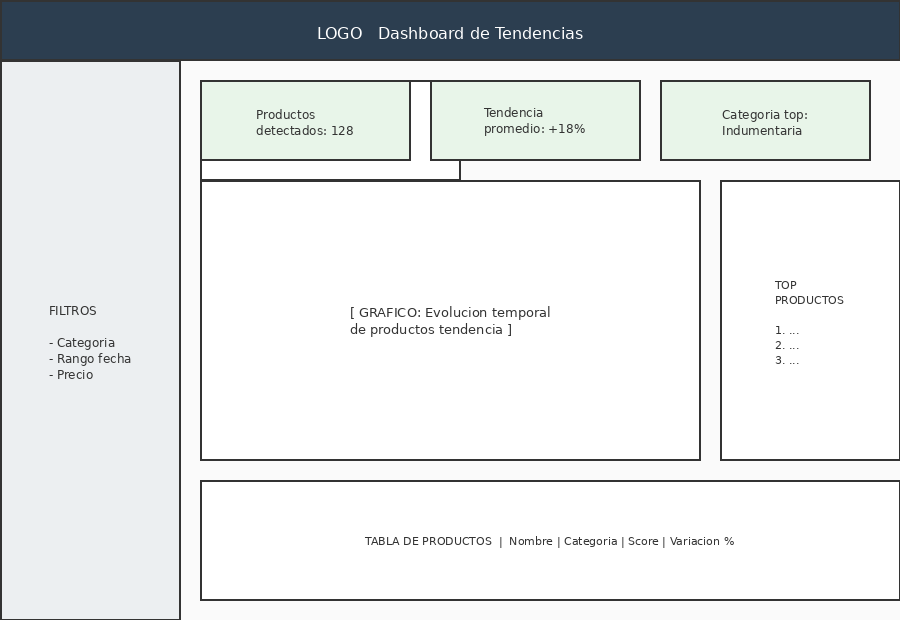
\includegraphics[width=0.85\textwidth]{./images/wireframes/wireframe_dashboard.png}
	\caption{Wireframe del Dashboard: filtros, KPIs, gráfico de tendencia y tabla de productos.}
	\label{fig:wireframe-dashboard}
\end{figure}

\section{Wireframe -- Detalle de producto}

\begin{figure}[H]
	\centering
	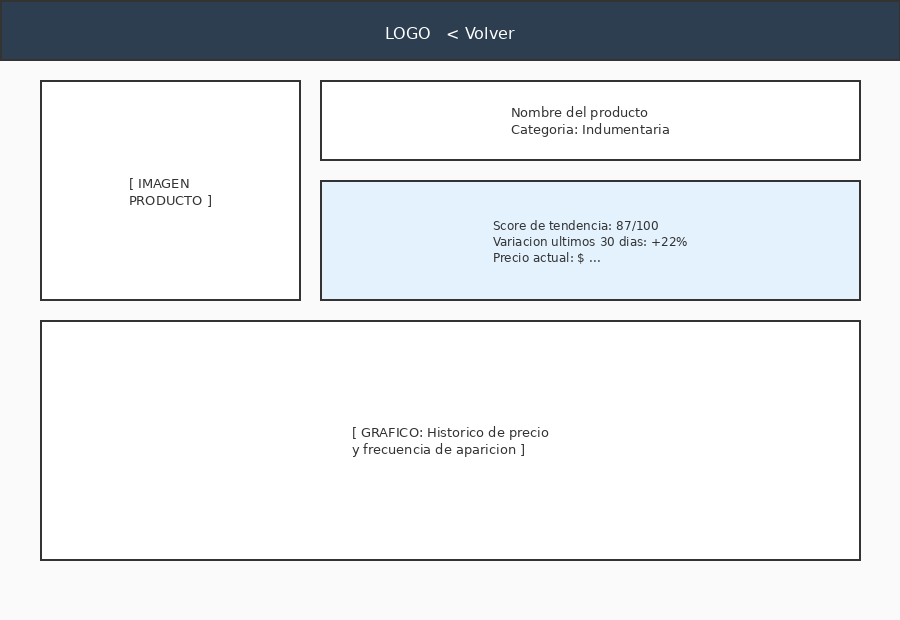
\includegraphics[width=0.85\textwidth]{./images/wireframes/wireframe_detalle.png}
	\caption{Wireframe de la pantalla de detalle: score de tendencia, variación e histórico.}
	\label{fig:wireframe-detalle}
\end{figure}
 % Mockups
	\chapter{Competencias y Estrategia de Mercado}\label{chapter05}

Se aplican herramientas de análisis estratégico para posicionar el proyecto frente a la competencia. Este capítulo es complementario al núcleo técnico-investigativo del PFI (arquitectura y score de tendencia en el Capítulo 1, requerimientos en el Capítulo 3, User Research en el Capítulo 6 y validación empírica en el Capítulo 7): aporta contexto de mercado, pero no reemplaza ni condiciona las decisiones técnicas del sistema.

\section{Análisis FODA}

\begin{table}[ht]
	\centering
	\caption{Análisis FODA -- Fortalezas y Debilidades}
	\label{tab:foda-fd}
	\begin{tabularx}{\textwidth}{@{}X X@{}}
		\toprule
		\textbf{Fortalezas} & \textbf{Debilidades} \\
		\midrule
		Uso de API oficial (datos confiables y legales). Score de tendencia propio basado en histórico. &
		Dependencia de límites de la API oficial. Sin datos de otras plataformas (solo Mercado Libre). \\
		\bottomrule
	\end{tabularx}
\end{table}

\begin{table}[ht]
	\centering
	\caption{Análisis FODA -- Oportunidades y Amenazas}
	\label{tab:foda-oa}
	\begin{tabularx}{\textwidth}{@{}X X@{}}
		\toprule
		\textbf{Oportunidades} & \textbf{Amenazas} \\
		\midrule
		Creciente uso de marketplaces en Argentina. Vendedores sin herramientas de anticipación de demanda. &
		Cambios en política de acceso a la API de Mercado Libre. Aparición de herramientas similares por parte de la propia plataforma. \\
		\bottomrule
	\end{tabularx}
\end{table}

\section{Cruz de Porter (5 fuerzas)}

\begin{itemize}
	\item \textbf{Rivalidad entre competidores}: media -- existen soluciones genéricas (Google Trends) pero ninguna enfocada en Mercado Libre Argentina.
	\item \textbf{Poder de negociación de clientes}: alto -- vendedores pueden optar por no usar ninguna herramienta y decidir de forma manual.
	\item \textbf{Poder de negociación de proveedores}: alto -- el proyecto depende completamente de la API oficial de Mercado Libre.
	\item \textbf{Amenaza de nuevos entrantes}: media -- la barrera técnica es moderada, pero la especialización en el marketplace local es un diferencial.
	\item \textbf{Amenaza de productos sustitutos}: media -- hojas de cálculo manuales o seguimiento intuitivo por parte de vendedores.
\end{itemize}

\begin{figure}[H]
	\centering
	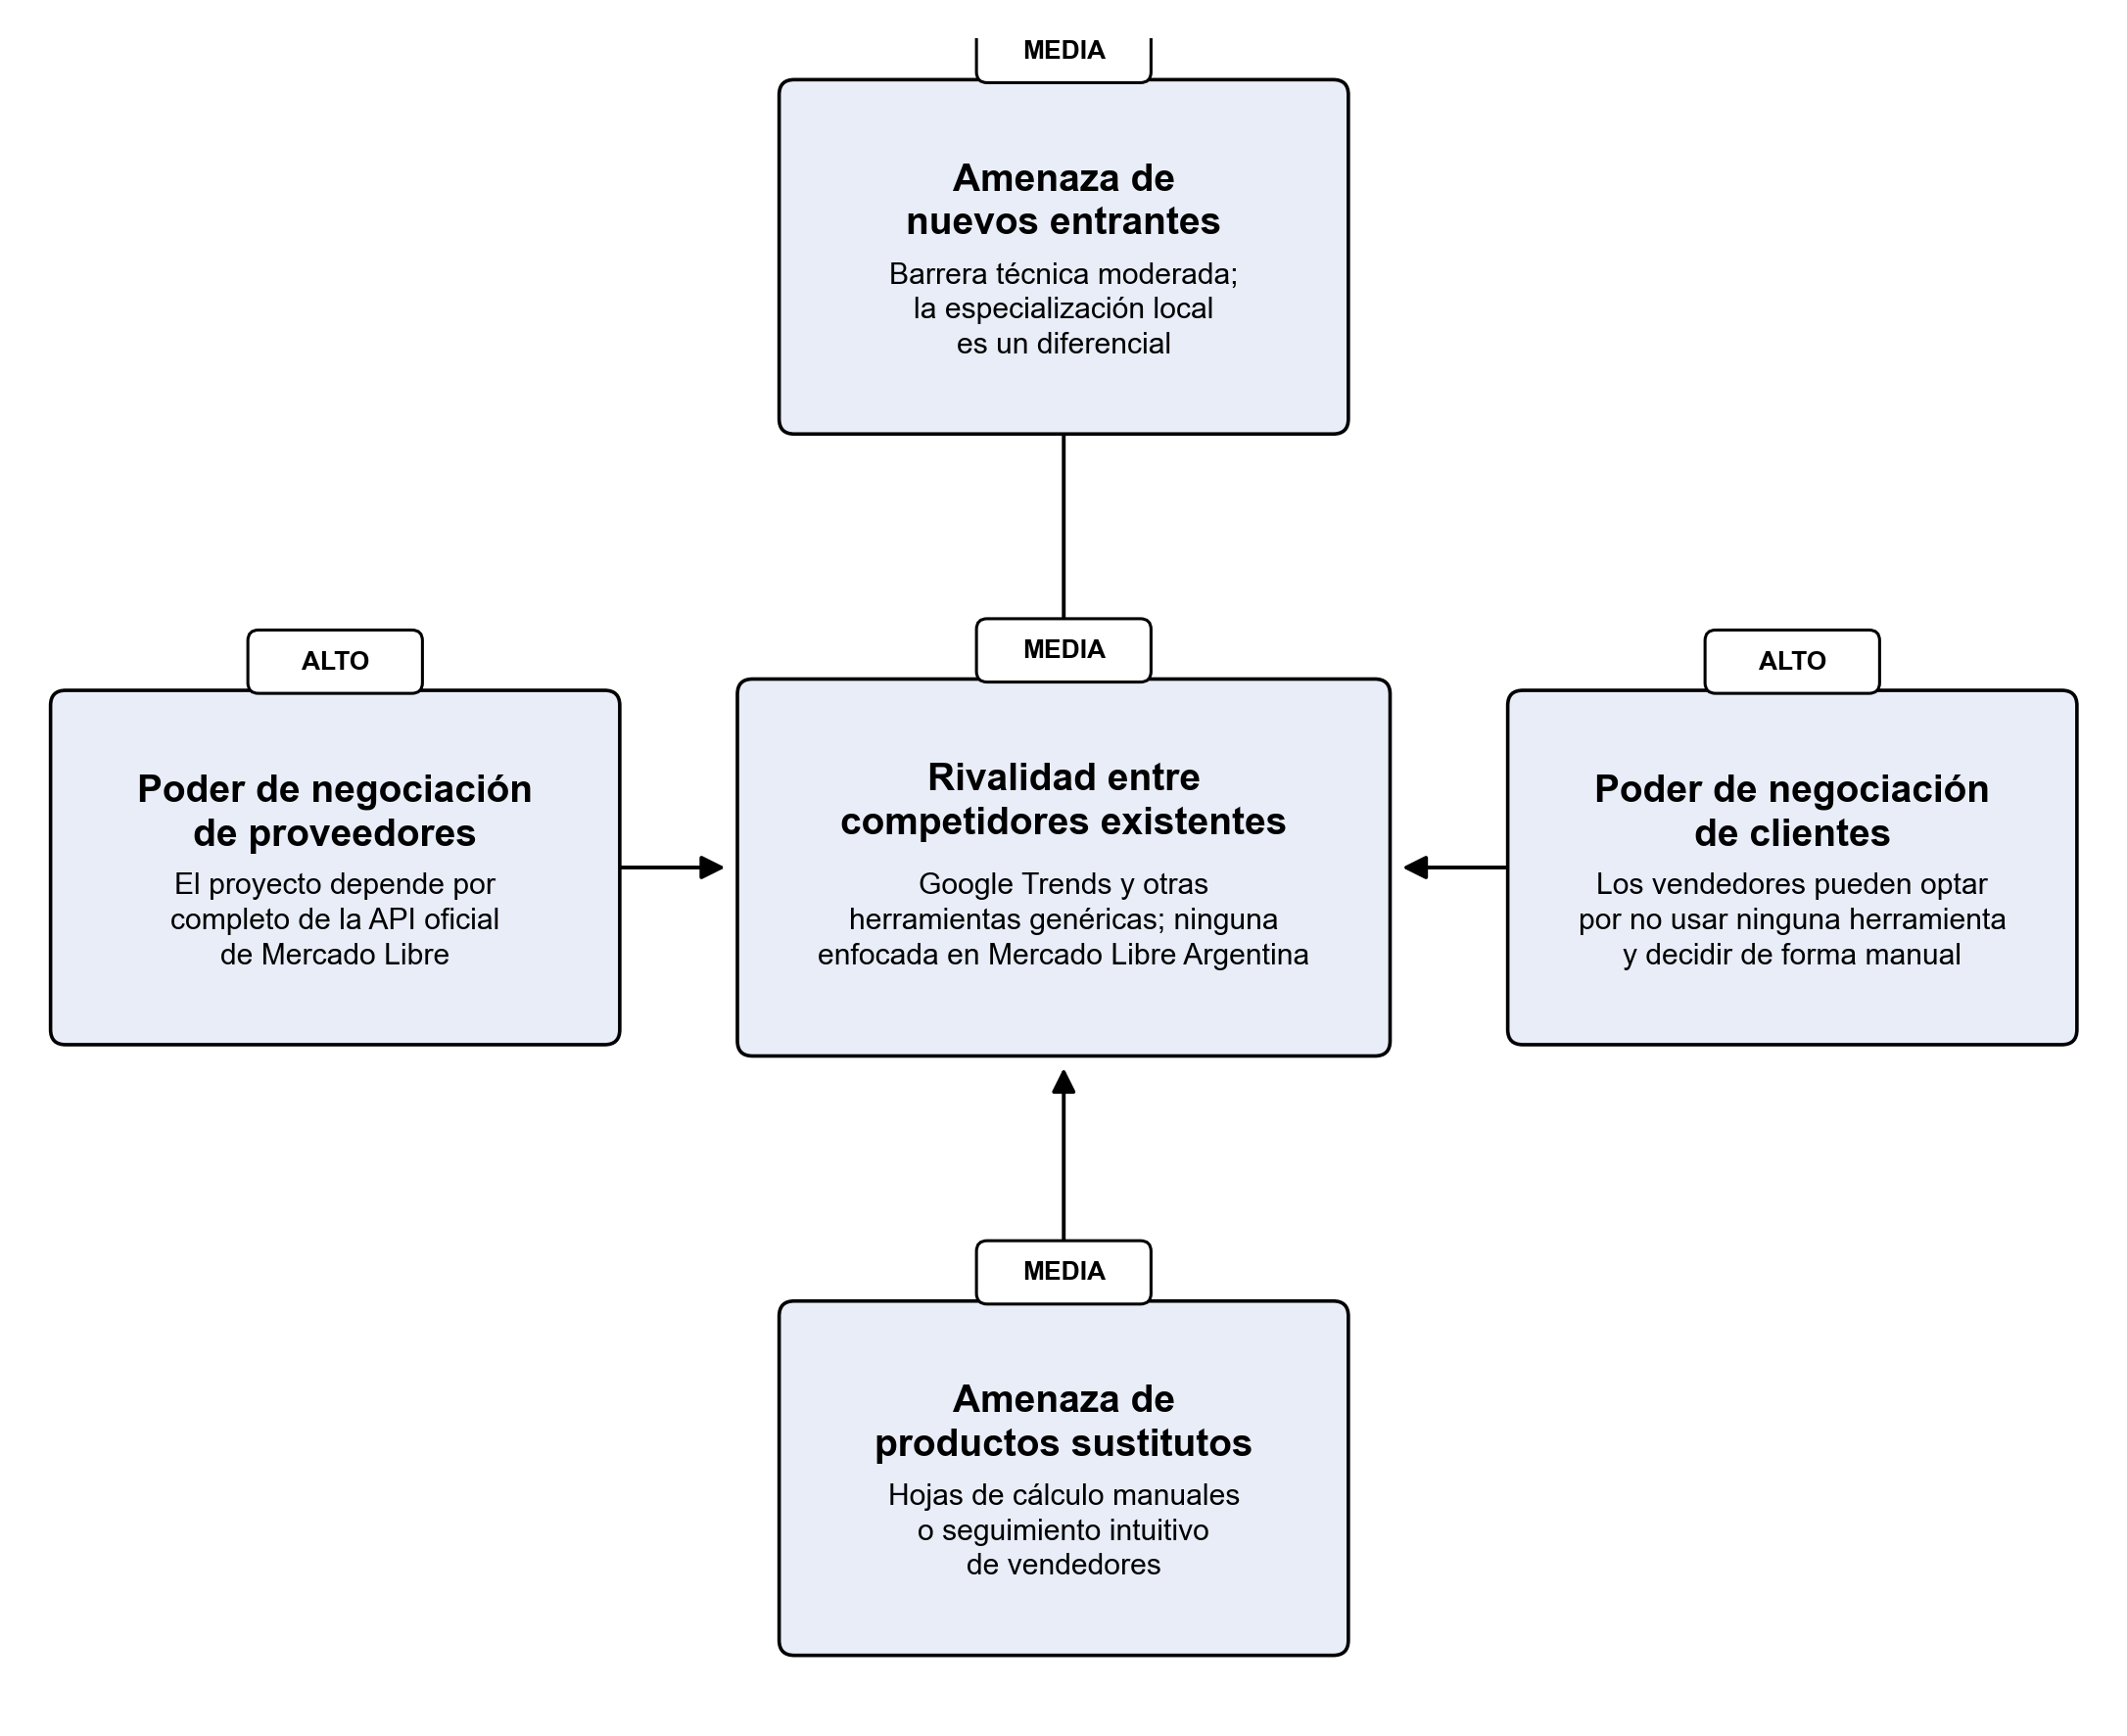
\includegraphics[width=0.95\textwidth]{./images/diagramas/diagrama_porter.png}
	\caption{Cruz de Porter (5 fuerzas) aplicada al proyecto.}
	\label{fig:diagrama-porter}
\end{figure}

\section{Triple P (Producto, Precio, Plaza)}

\begin{itemize}
	\item \textbf{Producto}: plataforma de detección temprana de productos en tendencia dentro de Mercado Libre, con dashboard y alertas.
	\item \textbf{Precio}: modelo freemium -- funciones básicas gratuitas y alertas/segmentación avanzada bajo suscripción mensual (desarrollado en la Sección~\ref{sec:modelo-negocio}).
	\item \textbf{Plaza}: acceso vía web, dirigido a vendedores PyME y particulares que operan en Mercado Libre Argentina.
\end{itemize}

\section{Modelo de negocio}\label{sec:modelo-negocio}

El modelo de negocio se apoya en el mismo segmento validado por el User Research (Capítulo~\ref{chapter06}): vendedores de Mercado Libre que hoy deciden qué stockear de forma intuitiva y manifestaron, en la encuesta, una disposición alta a adoptar una herramienta automatizada (68,9\,\% respondió ``Sí'' y 26,7\,\% ``Tal vez'').

\textbf{Propuesta de valor}: reducir el costo de detectar tarde una tendencia -- cuantificado por el vendedor entrevistado en una relación de rentabilidad de 3 a 1 respecto de haber tenido la señal dos semanas antes (Entrevista 1, Anexo D) -- mediante alertas y un score de tendencia auditable, en lugar de un ranking genérico sin desglose.

\textbf{Segmentos}: (a) vendedores individuales y PyME de Mercado Libre Argentina, segmento primario validado por la encuesta y las tres entrevistas; (b) agencias o gestores que administran varias cuentas de venta, como segmento secundario a explorar en una etapa posterior, sin validación propia todavía.

\textbf{Flujos de ingreso}: modelo freemium por suscripción mensual. El nivel gratuito ofrece el ranking y el dashboard con alcance acotado; el nivel pago -- validado en la Entrevista 2 en un rango de USD 10 a 30 mensuales (Anexo D) -- desbloquea alertas en tiempo real, historial completo y exportación sin límites.

\textbf{Canales}: adquisición orgánica a través de las mismas comunidades que ya usan los vendedores para intercambiar información. El grupo de WhatsApp de vendedores mencionado en la Entrevista 1 es, en los propios términos del entrevistado, el canal que más le aportó de todos los que probó, por encima de planillas propias o de seguir cuentas -- una señal directa de por dónde captar los primeros usuarios.

\textbf{Estructura de costos}: infraestructura cloud gestionada (Render y Supabase, Sección~\ref{sec:evidencia-cuantitativa}), comisión de la pasarela de pago sobre los ingresos, y un presupuesto de soporte y marketing continuo. No se contempla costo de personal más allá del equipo fundador actual.

\textbf{Sustentabilidad}: al ser un producto de software con costo marginal casi nulo por usuario adicional -- la infraestructura actual ya sostiene 162 productos y 3911 scores calculados sin necesidad de escalar (Sección~\ref{sec:evidencia-cuantitativa}) --, el margen de contribución por suscriptor es alto una vez cubiertos los costos fijos. El punto de equilibrio y los escenarios de rentabilidad se desarrollan en la Sección~\ref{sec:viabilidad-economica}.

\section{Viabilidad económico-financiera}\label{sec:viabilidad-economica}

Se evalúa la viabilidad económica del modelo de negocio mediante punto de equilibrio, Valor Actual Neto (VAN), Tasa Interna de Retorno (TIR) y período de recupero (\emph{payback}), sobre un horizonte de 24 meses y bajo los siguientes supuestos declarados:

\begin{itemize}
	\item \textbf{Precio de suscripción}: USD 15 mensuales, dentro del rango de USD 10 a 30 que el vendedor entrevistado consideró razonable (Entrevista 2, pregunta 9, Anexo D), elegido en el extremo conservador del rango.
	\item \textbf{Costos fijos mensuales}: USD 32 de infraestructura (Render y Supabase, según tarifas publicadas al momento de este informe -- a reverificar antes de la entrega final) más USD 60 de soporte y marketing continuo.
	\item \textbf{Costo variable}: comisión de pasarela de pago del 6\,\% sobre los ingresos por suscripción.
	\item \textbf{Inversión inicial}: USD 2000, que cubren identidad de marca, lanzamiento en las comunidades de vendedores identificadas como canal (Sección~\ref{sec:modelo-negocio}) y un colchón operativo de los primeros meses.
	\item \textbf{Tasa de descuento}: 1,5\,\% mensual (aprox. 18\,\% anual), consistente con el riesgo de un proyecto en etapa temprana en un mercado emergente.
	\item \textbf{Adopción}: dos escenarios de cantidad de suscriptores pagos, con una rampa lineal durante los primeros 6 meses y una meseta estable después. No se proyecta a partir del tamaño total del universo de vendedores de Mercado Libre Argentina, ya que no se dispone de una fuente pública confiable de esa cifra al momento de este informe -- los escenarios se construyen como cotas razonables (piso y techo) y no como una estimación de participación de mercado.
\end{itemize}

\begin{table}[H]
	\centering
	\caption{Escenarios de viabilidad económica}
	\label{tab:viabilidad-economica}
	\begin{tabularx}{\textwidth}{@{}>{\raggedright\arraybackslash}p{4.4cm} X X@{}}
		\toprule
		\textbf{Indicador} & \textbf{Pesimista} (meseta: 40 suscriptores) & \textbf{Optimista} (meseta: 150 suscriptores) \\
		\midrule
		Punto de equilibrio & \multicolumn{2}{p{7.6cm}}{7 suscriptores pagos por mes (cubre los USD 92 de costos fijos mensuales)} \\
		Flujo neto mensual en meseta & USD 472 & USD 2023 \\
		Período de recupero (\emph{payback}) & Mes 8 & Mes 4 \\
		VAN a 24 meses (tasa 1,5\,\% mensual) & USD 6092 & USD 33414 \\
		TIR mensual & 15,0\,\% & 45,7\,\% \\
		\bottomrule
	\end{tabularx}
\end{table}

Ambos escenarios muestran VAN positivo y recupero de la inversión inicial dentro del primer año, lo que respalda la viabilidad económica del modelo bajo los supuestos declarados. La TIR mensual es alta porque se trata de un producto de software con costo marginal casi nulo por usuario adicional y una inversión inicial acotada; por ese mismo motivo, anualizarla por interés compuesto produce un número con escaso valor interpretativo (una inversión inicial pequeña frente a un flujo de caja mensual sostenido infla artificialmente la tasa), por lo que se prioriza el VAN y el \emph{payback} como indicadores de decisión, en lugar de reportar esa TIR anualizada.

Como limitación del análisis, el modelo no proyecta el tamaño total del mercado direccionable -- no existe, al momento de este informe, una fuente pública confiable sobre el número de vendedores activos de Mercado Libre en Argentina -- ni incluye costo de personal más allá del equipo fundador actual. Ambos supuestos deberán revisarse si el proyecto avanza hacia una operación comercial real.

\section{Branding y logotipo}

\textbf{Nombre}: el producto se identifica comercialmente como \textbf{Tendar} -- de ``tendencia'' + ``radar'' --, elegido deliberadamente sin ninguna referencia a Mercado Libre en el nombre. Esta decisión responde a una observación de la instancia de revisión oral del hito del 50\,\%: atar la marca al nombre de la plataforma sobre la que opera hoy dejaría al producto sin identidad propia ante un cambio en las condiciones de acceso a esa API, riesgo ya identificado en el análisis FODA (Tabla~\ref{tab:foda-oa}) y en la Cruz de Porter (Figura~\ref{fig:diagrama-porter}). El título académico del proyecto (portada) se mantiene sin cambios, ya que corresponde a la Propuesta de Tema aprobada por la cátedra (Anexo A); Tendar es el nombre bajo el cual el producto se presentaría comercialmente.

\begin{figure}[H]
	\centering
	
\includegraphics[width=0.85\textwidth]{./images/diagramas/logo_tendar.png}
	\caption{Logotipo de Tendar.}
	\label{fig:logo-tendar}
\end{figure}

\textbf{Logotipo} (Figura~\ref{fig:logo-tendar}): el isotipo combina un radar -- círculos concéntricos con un sector de barrido -- con una línea de tendencia ascendente que se despega del punto detectado: una traducción visual directa de lo que hace el sistema, detectar una señal temprano (el radar) y mostrar que está despegando (la línea ascendente), en lugar de un ícono genérico de gráfico de barras o de carrito de compras. La paleta de azules es consistente con el resto de las figuras del documento (diagramas de arquitectura, Cruz de Porter), para mantener una identidad visual única entre el sistema y el informe que lo documenta.

\textbf{Tagline}: ``radar de tendencias'' -- resume la propuesta de valor (Sección~\ref{sec:modelo-negocio}) en tres palabras: detección (radar) del objeto central del negocio (tendencias).

\textbf{Tono de comunicación}: directo y cuantitativo, sin adjetivos vacíos, consistente con el hallazgo de la Entrevista 2 de que el score necesita explicabilidad para generar confianza (Sección~\ref{sec:pruebas}). La comunicación de marca evita promesas genéricas del tipo ``sabé lo que se viene'' y en cambio se apoya en números concretos -- el score, su desglose, el ejemplo real de la Sección~\ref{sec:score-formal} --, replicando en la comunicación la misma lógica de transparencia que ya tiene el producto.
 % Competencias y Estrategia de Mercado
	\chapter{User Research}\label{chapter06}

\section*{Introducción breve}

Con el objetivo de comprender las necesidades y problemáticas de potenciales usuarios vinculados al comercio electrónico, se realizó una instancia inicial de User Research orientada a emprendedores, revendedores digitales y usuarios interesados en la detección de tendencias comerciales.

La investigación tuvo como propósito identificar dificultades relacionadas con la búsqueda de productos emergentes, acceso a información histórica y utilización de herramientas de análisis dentro de plataformas ecommerce.

\section{Objetivo de la encuesta}

La encuesta fue diseñada para identificar hábitos de búsqueda de productos, dificultades para detectar tendencias y nivel de utilización de herramientas de análisis comercial.

El relevamiento se realizó mediante una encuesta digital elaborada en Google Forms entre el 26 de mayo y el 16 de julio de 2026 mediante un formulario combinado con preguntas cerradas, escalas de valoración de 1 a 5 y preguntas abiertas breves, permitiendo relevar tanto datos cuantitativos como comentarios cualitativos. El canal de difusión utilizado fue WhatsApp y además contactos personales. El criterio de selección fue no probabilístico por conveniencia, orientado a personas con interés en comercio electrónico, venta digital o compra de productos en marketplaces. Los gráficos completos de resultados generados por Google Forms se incluyen en el Anexo de Resultados de la Encuesta.

\subsection*{Fundamentación de la muestra}

Se obtuvieron 120 respuestas válidas. Para el análisis, las respuestas se segmentaron entre vendedores, compradores y participantes sin rol activo declarado. Las preguntas dirigidas a vendedores se utilizaron para validar la problemática principal de detección tardía de productos, mientras que las preguntas dirigidas a compradores se analizaron como señales complementarias de demanda, precio e influencia de redes sociales.

Como limitación metodológica, la muestra no es representativa de todo el universo de usuarios de Mercado Libre Argentina, ya que se concentra principalmente en CABA y Buenos Aires. Por ese motivo, los resultados se interpretan como exploratorios y útiles para orientar el diseño inicial de la plataforma.

\section{Composición de la muestra}

La primera pregunta permitió dividir a los participantes según su rol principal en Mercado Libre. Sobre 120 respuestas, el 37,5\% indicó ser vendedor, el 50,8\% comprador y el 11,7\% ninguna de las opciones. Esto equivale a 45 vendedores, 61 compradores y 14 participantes sin rol activo declarado.

\begin{table}[ht]
	\centering
	\caption{Composición de la muestra}
	\label{tab:composicion}
	\begin{tabularx}{0.7\textwidth}{@{}X c c@{}}
		\toprule
		\textbf{Rol declarado} & \textbf{Porcentaje} & \textbf{Cantidad aproximada} \\
		\midrule
		Vendedor & 37,5\% & 45 respuestas \\
		Comprador & 50,8\% & 61 respuestas \\
		Ninguna & 11,7\% & 14 respuestas \\
		Total & 100\% & 120 respuestas \\
		\bottomrule
	\end{tabularx}
\end{table}

Las preguntas específicas para vendedores registraron entre 43 y 45 respuestas, debido a que una de las preguntas del bloque vendedor registró dos respuestas menos. Las preguntas específicas para compradores registraron 61 respuestas.

\section{Resultados del segmento vendedor}

El bloque de vendedores permite observar el problema desde el punto de vista de quienes podrían utilizar directamente la plataforma propuesta para tomar decisiones de stock, detectar oportunidades comerciales y analizar tendencias antes de que se consoliden.

\begin{table}[ht]
	\centering
	\caption{Resultados del segmento vendedor}
	\label{tab:resultados-vendedor}
	\begin{tabularx}{\textwidth}{@{}>{\raggedright\arraybackslash}p{3.8cm} >{\raggedright\arraybackslash}p{5.5cm} X@{}}
		\toprule
		\textbf{Pregunta} & \textbf{Resultado principal} & \textbf{Interpretación} \\
		\midrule
		Dificultad para encontrar productos que puedan volverse tendencia & Sobre 43 respuestas, el 69,7\% eligió valores 4 o 5. El promedio fue 3,9 sobre 5. & Existe una dificultad alta para anticipar productos con potencial de tendencia. \\
		Método actual de detección & Tendencias dentro de Mercado Libre: 31,1\%; publicidad: 22,2\%; recomendaciones: 20\%; redes sociales: 13,3\%; otros: 13,3\%. & Los vendedores combinan varias fuentes, pero no aparece un método único ni sistemático. \\
		Percepción de detección tardía & 40\% respondió Sí, 48,9\% A veces y 11,1\% No. & La mayoría considera que las tendencias se detectan tarde o, al menos, no siempre a tiempo. \\
		Información más útil en una herramienta de análisis & Predicción de crecimiento: 28,9\%; competencia: 26,7\%; categorías de crecimiento: 20\%; historial de precios: 13,3\%; productos emergentes: 11,1\%. & La necesidad principal no es solo ver productos, sino anticipar crecimiento y analizar competencia. \\
		Disposición a usar una herramienta automatizada & 68,9\% respondió Sí, 26,7\% Tal vez y 4,4\% No. & Existe una aceptación alta de una solución automatizada para detectar productos emergentes. \\
		\bottomrule
	\end{tabularx}
\end{table}

\section{Resultados del segmento comprador}

El bloque comprador permite analizar señales de comportamiento del lado de la demanda. Aunque el usuario principal de la plataforma puede ser el vendedor o emprendedor, entender qué motiva a los compradores ayuda a definir qué variables y visualizaciones pueden resultar relevantes.

\begin{table}[ht]
	\centering
	\caption{Resultados del segmento comprador}
	\label{tab:resultados-comprador}
	\begin{tabularx}{\textwidth}{@{}>{\raggedright\arraybackslash}p{3.8cm} >{\raggedright\arraybackslash}p{5.5cm} X@{}}
		\toprule
		\textbf{Pregunta} & \textbf{Resultado principal} & \textbf{Interpretación} \\
		\midrule
		Motivación para comprar productos nuevos o novedosos & Recomendaciones: 26,2\%; redes sociales: 21,3\%; novedad: 19,7\%; precio: 16,4\%; publicidad: 16,4\%. & Las señales sociales (recomendaciones y redes) desplazan al precio como factor principal en la compra de productos novedosos, hallazgo relevante para las variables del modelo. \\
		Percepción de resultados repetidos en Mercado Libre & El 36,1\% eligió 5, el 23\% eligió 4, el 24,6\% eligió 3, el 14,8\% eligió 2 y el 1,5\% eligió 1. Promedio aproximado: 3,8 sobre 5. & Existe una percepción alta de repetición o concentración de resultados destacados (el 59,1\% eligió valores 4 o 5). \\
		Influencia de TikTok e Instagram & Promedio aproximado: 3,3 sobre 5. El 47,5\% eligió valores 4 o 5. & La influencia de redes sociales es moderada, pero relevante como señal complementaria para entender demanda. \\
		\bottomrule
	\end{tabularx}
\end{table}

\section{Resultados generales}

\begin{table}[ht]
	\centering
	\caption{Resultados generales}
	\label{tab:resultados-generales}
	\begin{tabularx}{\textwidth}{@{}>{\raggedright\arraybackslash}p{2.5cm} >{\raggedright\arraybackslash}p{6cm} X@{}}
		\toprule
		\textbf{Variable} & \textbf{Resultado} & \textbf{Lectura} \\
		\midrule
		Rango de edad & 18 a 30: 43,3\%; 31 a 50: 40,8\%; más de 50: 10,8\%; menos de 18: 5,1\%. & La muestra se concentra principalmente en adultos jóvenes y adultos en edad laboral. \\
		Ubicación & Sobre 119 respuestas, se agruparon variantes escritas manualmente: Buenos Aires / Provincia de Buenos Aires aprox. 40\%; CABA aprox. 28\%; respuestas genéricas (``Argentina'') u otras provincias aprox. 32\%. & La muestra se concentra en CABA y Buenos Aires, lo cual debe considerarse como una limitación del relevamiento. \\
		Comentarios abiertos & Aparecieron menciones a comparación de precios, opiniones del vendedor, recomendación de productos nuevos y necesidad de una herramienta visual. & Los comentarios refuerzan la utilidad de una plataforma visual, orientada a precios, recomendaciones y análisis comercial. \\
		\bottomrule
	\end{tabularx}
\end{table}

\section{Principales datos obtenidos}

\begin{itemize}
	\item Existe una dificultad alta para anticipar productos tendencia: el 69,7\% de los vendedores que respondieron esa pregunta seleccionó valores 4 o 5.
	\item La detección tardía aparece como un problema relevante: el 40\% respondió que las tendencias muchas veces se detectan demasiado tarde y el 48,9\% respondió que eso ocurre a veces (88,9\% combinado).
	\item La aceptación de una herramienta automatizada es alta: el 68,9\% de los vendedores indicó que la usaría y un 26,7\% adicional respondió ``tal vez'' (solo el 4,4\% la descartó).
	\item Los vendedores valoran especialmente la predicción de crecimiento y el análisis de competencia, lo que refuerza la necesidad de una plataforma que no se limite a mostrar rankings actuales.
	\item Desde el lado comprador, las recomendaciones (26,2\%) y las redes sociales (21,3\%) aparecen como los factores principales de decisión, seguidas por la novedad (19,7\%) y el precio (16,4\%); esto refuerza el valor de las señales sociales como variables complementarias para interpretar oportunidades comerciales.
	\item La muestra se concentra en CABA y Buenos Aires, por lo que los resultados deben entenderse como exploratorios y no generalizables a todo el país.
\end{itemize}

Los resultados obtenidos respaldan la problemática inicial del proyecto. Los vendedores manifiestan dificultad para anticipar tendencias, perciben que muchas oportunidades se detectan tarde y muestran alta disposición a utilizar una herramienta automatizada. Al mismo tiempo, los compradores confirman la influencia de variables como recomendaciones, redes sociales y precio. En conjunto, estos hallazgos justifican el desarrollo de una plataforma orientada a detectar productos emergentes mediante históricos, métricas temporales y visualización analítica.

\section{Entrevistas en profundidad}

Como complemento cualitativo de la encuesta, se diseñaron tres entrevistas semiestructuradas a usuarios reales de Mercado Libre: dos vendedores y un comprador, seleccionados por muestreo intencional entre personas con actividad verificable en la plataforma (no se buscan perfiles profesionales ni expertos, sino usuarios comunes, en línea con el público objetivo de la herramienta). El propósito es profundizar en el porqué de los patrones cuantitativos observados en la encuesta: la detección tardía de tendencias (88,9\% combinado), la alta disposición a usar una herramienta automatizada (68,9\%) y el peso de las señales sociales en la decisión de compra (47,5\%). Cada entrevista dura entre 20 y 30 minutos, se registra con consentimiento informado y se analiza mediante síntesis temática. Los hallazgos se integrarán a esta sección una vez realizadas las entrevistas. El diseño completo de las tres guías de entrevista (objetivos y las 10 preguntas de cada una) se incluye en el Anexo de Entrevistas.

\section{User persona}

A partir de los hallazgos reales de la encuesta se construyen dos user personas preliminares. No representan personas individuales encuestadas, sino perfiles sintéticos elaborados a partir de patrones observados en las respuestas. Su objetivo es conectar los resultados del relevamiento con necesidades concretas de diseño de la plataforma.

\subsection*{User Persona 1: Martín, vendedor que necesita anticiparse}

\begin{table}[ht]
	\centering
	\caption{User Persona 1 -- Martín}
	\label{tab:persona-martin}
	\begin{tabularx}{\textwidth}{@{}>{\raggedright\arraybackslash}p{3cm} X@{}}
		\toprule
		\textbf{Campo} & \textbf{Descripción} \\
		\midrule
		Perfil & Martín tiene 29 años, vive en Buenos Aires y vende productos por Mercado Libre. Representa al segmento vendedor de la encuesta, que declaró dificultades altas para encontrar productos que puedan volverse tendencia. Tiene experiencia básica/intermedia en ventas online y consulta distintas fuentes antes de decidir qué productos incorporar. \\
		Necesidad & Necesita detectar productos con potencial de crecimiento antes de que se consoliden y antes de que aumente demasiado la competencia. También necesita comparar la evolución del producto con su categoría para evitar decisiones basadas solo en una aparición aislada. \\
		Frustración & Siente que muchas veces llega tarde a las tendencias: cuando identifica un producto atractivo, ya existen muchos vendedores ofreciendo lo mismo y los márgenes se reducen. \\
		Objetivo & Tomar decisiones de stock con más información, priorizando productos que muestren crecimiento sostenido y señales tempranas de demanda. \\
		Relación con la plataforma propuesta & Sería un usuario directo del dashboard. Consultaría productos emergentes, predicción de crecimiento, evolución de precios y nivel de competencia para decidir qué vender o qué analizar con mayor profundidad. La plataforma le permitiría priorizar oportunidades según señales históricas, no solamente según intuición o publicaciones virales. \\
		\bottomrule
	\end{tabularx}
\end{table}

\subsection*{User Persona 2: Luciana, compradora digital con comportamiento influido por precio y redes}

\begin{table}[ht]
	\centering
	\caption{User Persona 2 -- Luciana}
	\label{tab:persona-luciana}
	\begin{tabularx}{\textwidth}{@{}>{\raggedright\arraybackslash}p{3cm} X@{}}
		\toprule
		\textbf{Campo} & \textbf{Descripción} \\
		\midrule
		Perfil & Luciana tiene 32 años, vive en CABA y compra habitualmente en Mercado Libre. Representa al segmento comprador de la encuesta, donde las recomendaciones y las redes sociales aparecen como los factores más relevantes para decidir compras de productos novedosos. Su comportamiento representa señales indirectas de demanda que los vendedores pueden observar para interpretar interés de mercado. \\
		Necesidad & Quiere encontrar productos nuevos o convenientes sin depender únicamente de resultados destacados repetidos o recomendaciones superficiales. Necesita contar con información clara que le permita distinguir entre productos realmente convenientes y productos destacados solo por visibilidad comercial. \\
		Frustración & Percibe que muchas veces aparecen los mismos productos destacados y que no siempre es fácil comparar alternativas, precios u opiniones del vendedor. \\
		Objetivo & Comprar productos novedosos o recomendados con mayor confianza, comparando precio, reputación y señales de interés real. \\
		Relación con la plataforma propuesta & Aunque no sería necesariamente la usuaria principal del sistema, su comportamiento ayuda a definir qué señales de demanda deberían observar los vendedores: precio, redes sociales, recomendaciones y aparición repetida de productos. Sus hábitos permiten definir variables complementarias para el sistema, especialmente precio, repetición de publicaciones, reputación y presencia en redes sociales. \\
		\bottomrule
	\end{tabularx}
\end{table}

\section{Diagrama de Gantt}

El cronograma de actividades del proyecto se presenta en el Anexo de Cronograma de Actividades.

\section{Gestión de datasets}

El dataset del proyecto será construido de manera propia a partir de consultas periódicas a la API oficial de Mercado Libre Argentina. No se utilizará scraping, fuentes no autorizadas ni datos privados de usuarios. Los datos crudos provendrán de información pública disponible mediante endpoints oficiales, principalmente publicaciones, categorías, precios y atributos asociados a productos.

En esta etapa inicial, el volumen del dataset se plantea como estimado, ya que el histórico comenzará a construirse durante el desarrollo del prototipo. Primero se trabajará con una muestra controlada de productos y categorías, y luego podrá ampliarse incorporando mayor frecuencia de captura y más registros temporales.

La confiabilidad del origen se basa en el uso de la API oficial de Mercado Libre. Los datos serán almacenados en PostgreSQL para conservar registros estructurados y permitir comparaciones entre distintos períodos.

El tratamiento preliminar incluirá control de duplicados, validación de campos obligatorios, revisión de valores nulos, normalización de categorías y registro de fecha y hora de captura. De manera preliminar, se considerarán variables como identificador de publicación, título, categoría, precio, fecha de captura, frecuencia de aparición y cantidad de publicaciones asociadas.

Como limitación inicial, el proyecto no contará con históricos previos provistos por Mercado Libre. Por eso, el valor del dataset aumentará a medida que el sistema acumule registros en el tiempo.
 % User Research
	\chapter{Demo -- Avances de Implementación}\label{chapter07}

A continuación se presentan capturas del sistema en funcionamiento (agosto de 2026), correspondientes al avance de implementación de este hito del 75\%: el pipeline de captura y su monitoreo, la base de datos histórica, la API REST y el dashboard con el ranking por score de tendencia. El sistema se encuentra publicado y accesible en producción, con captura de datos automatizada ejecutándose de manera autónoma varias veces por día. La interfaz web se divide en dos vistas: un panel para clientes (\texttt{/dashboard}), con el ranking de productos y la evolución del score en el tiempo, y un panel técnico interno (\texttt{/admin}) con el monitoreo de endpoints y los registros de minería, que se documenta a continuación como evidencia de RNF01.

\begin{figure}[ht]
	\centering
	
\includegraphics[width=0.75\textwidth]{./images/demo/demo_dashboard.png}
	\caption{Panel técnico interno del sistema en funcionamiento (agosto 2026).}
	\label{fig:demo-dashboard}
\end{figure}

\begin{figure}[ht]
	\centering
	
\includegraphics[width=0.9\textwidth]{./images/demo/demo_dashboard_apis.png}
	\caption{Panel de disponibilidad de endpoints (EndpointHealthLog): monitoreo registrado en cada sesión de minería.}
	\label{fig:demo-apis}
\end{figure}

\begin{figure}[ht]
	\centering
	
\includegraphics[width=0.85\textwidth]{./images/demo/demo_dashboard_score.png}
	\caption{Panel de clientes: ranking de productos por score de tendencia (RF02), con filtros por categoría y exportación CSV (RF03/RF06).}
	\label{fig:demo-score}
\end{figure}

\begin{figure}[ht]
	\centering
	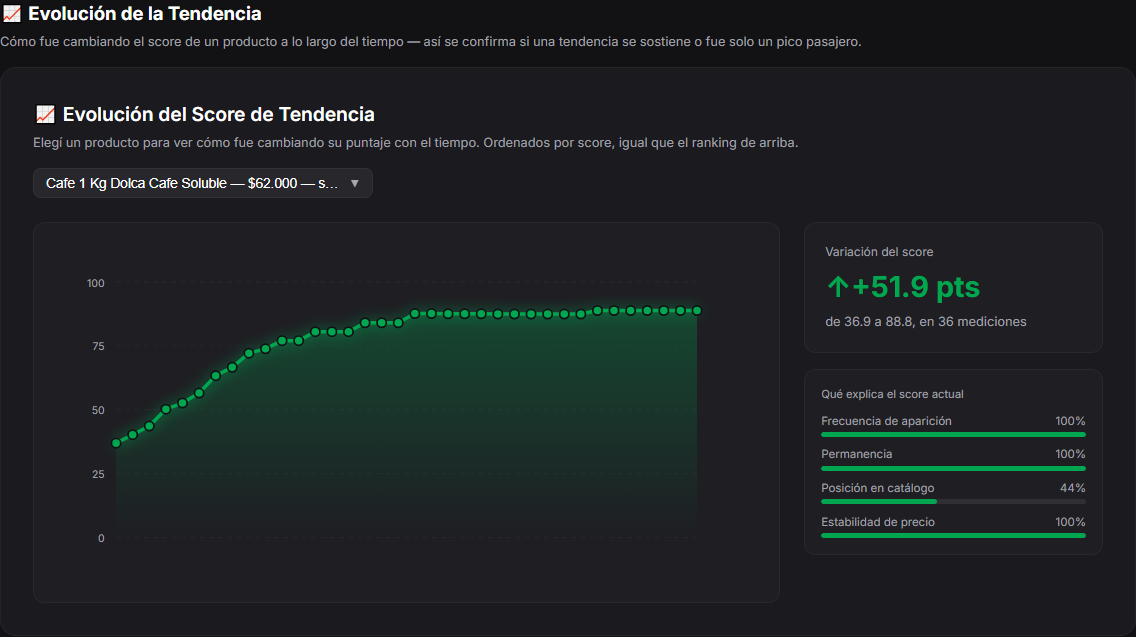
\includegraphics[width=0.85\textwidth]{./images/demo/demo_dashboard_evolucion.png}
	\caption{Panel de clientes: evolución del score de tendencia de un producto en el tiempo, con el desglose de sus componentes (RF02, RF05).}
	\label{fig:demo-evolucion}
\end{figure}

\section{Evidencia cuantitativa del sistema en producción}\label{sec:evidencia-cuantitativa}

Más allá de la afirmación de que el sistema está desplegado y capturando datos, esta sección documenta con números concretos, medidos directamente sobre la base de datos y los endpoints en producción, cómo se comporta el prototipo actual. Los volúmenes de datos se remidieron el 23/09/2026 para reflejar el crecimiento del histórico desde la primera medición (10/08/2026); los tiempos de respuesta mantienen la fecha de su propia medición, indicada en cada fila.

\begin{table}[H]
	\centering
	\small
	\caption{Métricas del sistema en producción (volúmenes de datos medidos el 23/09/2026)}
	\label{tab:evidencia}
	\begin{tabularx}{\textwidth}{@{}>{\raggedright\arraybackslash}p{5.2cm} X@{}}
		\toprule
		\textbf{Indicador} & \textbf{Valor medido} \\
		\midrule
		Rango temporal del histórico & 14/07/2026 -- 23/09/2026 (71 días de operación continua) \\
		Productos monitoreados & 274 \\
		Categorías monitoreadas & 6 (Computación, Celulares, Electrónica, Ropa y Accesorios, Alimentos y Bebidas, Limpieza del Hogar) \\
		Apariciones registradas (\texttt{TrendSnapshot}) & 5717 \\
		Registros de precio (\texttt{PriceHistory}) & 5807 \\
		Scores de tendencia calculados (\texttt{TrendScore}) & 11539 \\
		Registros de monitoreo de endpoints (\texttt{EndpointHealthLog}) & 1899 \\
		Sesiones de minería estimadas & $\sim$203 (agrupando snapshots por cortes de inactividad $>$40 min), $\sim$28,2 apariciones registradas por sesión en promedio \\
		Frecuencia de captura configurada & 3 corridas diarias (cron programado, ver Sección~\ref{sec:evolucion-tecnica}) \\
		Tiempo de respuesta -- \texttt{/api/health}, \texttt{/api/status} & 0,5 -- 2,1\,s (medido, 3 muestras c/u) \\
		Tiempo de respuesta -- \texttt{/dashboard} (panel de clientes) & 0,5 -- 1,1\,s en caliente (medido, 5 muestras el 15/08/2026, tras separar el panel de clientes del panel técnico) \\
		Tiempo de respuesta -- \texttt{/admin} (panel técnico) & 1,9 -- 4,0\,s (medido, 3 muestras el 15/08/2026) \\
		Tiempo de respuesta -- \texttt{/api/trend-scores} & 1,7 -- 2,9\,s en caliente (medido, 5 muestras el 21/09/2026, tras la corrección de RNF02 -- ver Sección~\ref{sec:pruebas}) \\
		\bottomrule
	\end{tabularx}
\end{table}

Un ejemplo real de exportación CSV (RF06) generado desde el dashboard el mismo día incluye columnas \texttt{producto, categoria, precio, moneda, variacion\_pct, score, periodo, calculado, link}, con una fila por cada producto del ranking filtrado en pantalla al momento de la exportación (ver Figura~\ref{fig:demo-score}).

Un hallazgo temprano de esta medición (10/08/2026) fue que \texttt{/api/trend-scores} -- el endpoint que alimenta el ranking principal -- no cumplía el objetivo de RNF02 (respuesta en menos de 3 segundos): la consulta traía los 3911 scores históricos con sus relaciones completas en cada solicitud, en lugar de traer solamente las últimas mediciones vigentes por producto. La corrección aplicada y su verificación posterior en producción se documentan en la Sección~\ref{sec:pruebas}.

\section{Pruebas funcionales y resultados}\label{sec:pruebas}

Sobre el sistema en producción se aplicaron dos técnicas de prueba distintas: pruebas de rendimiento sobre los requerimientos no funcionales, y una prueba de usabilidad embebida en una entrevista con un usuario real.

\subsection*{Pruebas de rendimiento (RNF02)}

La medición del 10/08/2026 (Tabla~\ref{tab:evidencia}) mostró que \texttt{/api/trend-scores} respondía en 6,3--7,6\,s, por encima del objetivo de 3\,s de RNF02. La causa identificada fue que la consulta traía el historial completo de \texttt{TrendScore} (más de 7700 filas a esa fecha) con el historial de precios de cada producto anidado, cuando el dashboard solo necesita las últimas 2 mediciones por producto para calcular la variación mostrada en pantalla. La corrección, aplicada acotando la consulta a esas últimas 2 mediciones, se verificó nuevamente en producción el 21/09/2026 con 5 muestras adicionales: el tiempo de respuesta bajó a 1,7--2,9\,s en caliente, dentro del objetivo. RNF02 pasa así de \emph{Parcial} a \emph{Implementado} en la matriz de trazabilidad (Sección~\ref{sec:trazabilidad}).

\subsection*{Prueba de usabilidad}

La Entrevista 2 (Anexo D, Sección~\ref{chapter06}) incluyó una instancia de prueba de usabilidad: se mostró el dashboard en funcionamiento a un vendedor real (Lucas) y se le pidió que interpretara la pantalla sin explicación previa (pregunta 3, ``¿Qué entendés que muestra esta pantalla?''). El entrevistado identificó correctamente el propósito del ranking y del score sin asistencia, lo que valida que la interfaz comunica su función principal sin necesidad de instrucciones adicionales.

Esa misma instancia motivó una decisión de diseño a partir de sus resultados: la pregunta sobre qué le faltaba a la herramienta (pregunta 8) y la objeción de que el score funcionaba como una ``caja negra'' (pregunta 10) llevaron a que el desglose de sus cuatro componentes -- frecuencia, permanencia, ranking, estabilidad -- se muestre explícitamente en el dashboard en lugar de solo el puntaje final, decisión ya documentada en la Sección~\ref{sec:score-formal}.
 % Demo - Avances de Implementación
	\chapter{Conclusi\'on}\label{conclussions}

\section{Resumen de aportes}

El objetivo general del proyecto (Sección~\ref{sec:objetivo-general}) fue desarrollar una plataforma capaz de detectar tempranamente productos emergentes en Mercado Libre, combinando captura automatizada, un histórico propio y análisis temporal con métricas descriptivas y modelos supervisados. Al cierre de este hito, los cinco objetivos específicos (Sección~\ref{sec:objetivos-especificos}) están cubiertos:

\begin{itemize}
	\item La captura automatizada y periódica (RF01) opera de forma autónoma desde el despliegue, con 274 productos y 71 días de histórico continuo acumulados sin intervención manual (Sección~\ref{sec:evidencia-cuantitativa}).
	\item El score de tendencia (RF02) quedó formalizado con una fórmula auditable de cinco componentes ponderados -- el quinto, saturación por cantidad de vendedores, incorporado directamente a partir de la devolución del jurado y de lo que describieron los propios vendedores entrevistados sobre detectar oportunidades antes de que se saturen de oferta --, validada con ejemplos reales del sistema (Sección~\ref{sec:score-formal}) y con su desglose expuesto en el dashboard -- decisión tomada directamente a partir de un hallazgo de la Entrevista 2 (Sección~\ref{sec:pruebas}).
	\item El dashboard de filtrado y ordenamiento (RF03), la API REST (RF04), los gráficos de evolución temporal (RF05) y la exportación CSV (RF06) están implementados y verificados en producción, según documenta la matriz de trazabilidad (Sección~\ref{sec:trazabilidad}).
	\item Las bases metodológicas para el modelo supervisado no solo quedaron sentadas, sino que se ejecutaron como un primer checkpoint entrenado y evaluado: un Random Forest con \emph{recall} de 0,807 y AUC-ROC de 0,903 sobre el histórico disponible (Sección~\ref{sec:ml-resultados}), con la variable más relevante (aceleración de la frecuencia de aparición) siendo interpretable y consistente con el criterio que describieron los propios vendedores entrevistados.
\end{itemize}

Además de esos cinco objetivos, se incorporaron tres funcionalidades no contempladas en el diseño original (RF07--RF09, Sección~\ref{sec:demo-cuentas}), a partir de la devolución del jurado de que el sistema se leía como un simple dashboard: la probabilidad del modelo de ML visible por producto en el ranking, un sistema de cuentas que diferencia un nivel gratuito de uno pago (freemium, ya real y no solo planificado, Sección~\ref{sec:modelo-negocio}), y alertas dentro de la aplicación para productos seguidos, que resuelven HU02 de la forma en que los propios vendedores entrevistados pidieron que se resolviera: avisando, no obligando a revisar el panel.

Más allá de los requerimientos funcionales, el proyecto aporta evidencia de que la problemática elegida es real y no supuesta: el 88,9\,\% de los vendedores encuestados reconoce detectar tendencias tarde o solo a veces a tiempo, y el 68,9\,\% adoptaría una herramienta automatizada para resolverlo (Capítulo~\ref{chapter06}). Las tres entrevistas en profundidad no solo confirmaron estos números de forma cualitativa, sino que moldearon decisiones de diseño concretas y verificables en el sistema: la explicabilidad del score, la prioridad de las alertas por sobre la consulta manual, y el peso de la permanencia temporal en la fórmula.

El proyecto también deja resuelto lo que en la instancia de revisión oral del hito del 50\,\% se señaló como insuficiente para un trabajo de esta envergadura: un modelo de negocio desarrollado con viabilidad económica cuantificada en dos escenarios (Sección~\ref{sec:viabilidad-economica}), una identidad de marca propia e independiente de Mercado Libre (Tendar, Sección~\ref{sec:modelo-negocio}), y la resolución -- no solo documentada, sino implementada en el modelo de datos y probada -- de a qué se refiere el sistema cuando habla de ``un producto'' ante la ambigüedad de que un mismo modelo lo vendan simultáneamente decenas de vendedores distintos: la identidad de cada producto pasó a anclarse al identificador de catálogo de Mercado Libre en lugar de a la publicación puntual del vendedor más barato del momento (Sección~\ref{sec:concepto-central}). Ninguno de estos tres puntos estaba resuelto en la entrega anterior; los tres se abordaron de forma honesta, incluyendo el reconocimiento explícito de sus límites en lugar de ocultarlos.

\section{Trabajo futuro}

\begin{itemize}
	\item \textbf{Reentrenamiento del modelo con más histórico}: el checkpoint actual (Sección~\ref{sec:ml-resultados}) cubre 71 días, todavía por debajo de los varios meses estimados como necesarios para observar ciclos completos de aparición-crecimiento-declive por categoría. El pipeline ya quedó versionado y es reejecutable sin cambios de diseño a medida que el histórico siga creciendo.
	\item \textbf{Envío real de alertas por email o push}: RF09 hoy resuelve HU02 como bandeja dentro de la aplicación (\texttt{/alerts}), pero no envía la notificación por fuera de la app. El mecanismo de detección y generación de alertas ya está construido (\texttt{scripts/generate\_alerts.js}); falta exclusivamente dar de alta una cuenta en un proveedor de correo externo para conectar el envío.
	\item \textbf{Pasarela de pago}: el nivel pago del modelo freemium (RF08) ya diferencia funciones reales entre cuenta gratuita y con sesión, pero el registro en sí es gratuito -- no hay cobro integrado todavía. Es el paso que falta para validar el modelo de negocio con datos de conversión reales en vez de supuestos.
	\item \textbf{Optimización continua de rendimiento}: RNF02 ya se corrigió una vez (de 6,3--7,6\,s a 1,7--2,9\,s, Sección~\ref{sec:pruebas}); a medida que el histórico crezca conviene monitorear que el tiempo de respuesta se mantenga dentro del objetivo.
	\item \textbf{Ampliación del alcance geográfico del User Research}: la encuesta y las entrevistas se concentraron en CABA y Buenos Aires (Capítulo~\ref{chapter06}); una muestra con mayor representación del resto del país fortalecería la validación de la problemática a nivel nacional.
	\item \textbf{Validación del modelo de negocio con usuarios reales}: los escenarios de viabilidad económica (Sección~\ref{sec:viabilidad-economica}) se construyeron sobre supuestos declarados y la disposición a pagar relevada en una sola entrevista; una prueba piloto con suscriptores reales permitiría reemplazar esos supuestos por datos de conversión efectivos.
\end{itemize}


	\addcontentsline{toc}{chapter}{Bibliograf\'{\i}a}
	% Incluye tambien las referencias metodologicas no citadas narrativamente
	% en el cuerpo del texto (Hernandez-Sampieri, Kitchenham, ML Developers).
	\nocite{*}
	\printbibliography{}

	\appendix
	% annex.tex ya incluye internamente schedule_of_activities, surveys e interviews
	% mediante el comando \anexo{} (no deben inputearse por separado).
	\input{chapters/appendix/annex}
	\newpage
	\listoffigures
	\newpage
	\listoftables
\end{document}
